%%% Local Variables:
%%% mode: latex
%%% TeX-master: t
%%% End:

\documentclass[bachelor]{thuthesis}
% \documentclass[%
%   bachelor|master|doctor|postdoctor, % mandatory option
%   xetex|pdftex|dvips|dvipdfm, % optional
%   secret,
%   openany|openright,
%   arialtoc,arialtitle]{thuthesis}

% 所有其它可能用到的包都统一放到这里了,可以根据自己的实际添加或者删除。
\usepackage{thutils}
\usepackage{lscape}

% 你可以在这里修改配置文件中的定义,导言区可以使用中文。
% \def\myname{徐驰}

\DeclareMathOperator\dif{d\!}
\newcolumntype{Y}{>{\centering\arraybackslash}X} 
\DeclareMathOperator{\amp}{Amp}



\begin{document}

% 定义所有的eps文件在 figures 子目录下
\graphicspath{{figures/}}


%%% 封面部分
\frontmatter

%%% Local Variables:
%%% mode: latex
%%% TeX-master: t
%%% End:
\secretlevel{绝密} \secretyear{2100}

\ctitle{保留在制品库存对安全库存的影响}
% 根据自己的情况选,不用这样复杂
\makeatletter
\ifthu@bachelor\relax\else
  \ifthu@doctor
    \cdegree{工学博士}
  \else
    \ifthu@master
      \cdegree{工学硕士}
    \fi
  \fi
\fi
\makeatother


\cdepartment[工业工程系]{工业工程系}
\cmajor{工业工程}
\cauthor{徐驰} 
\csupervisor{吴甦教授}
% 如果没有副指导老师或者联合指导老师,把下面两行相应的删除即可。
%\cassosupervisor{陈文光教授}
%\ccosupervisor{某某某教授}
% 日期自动生成,如果你要自己写就改这个cdate
%\cdate{\CJKdigits{\the\year}年\CJKnumber{\the\month}月}

% 博士后部分
% \cfirstdiscipline{计算机科学与技术}
% \cseconddiscipline{系统结构}
% \postdoctordate{2009年7月——2011年7月}

\etitle{The Impact of Reserving In-process Inventory on Safety Stock} 
% \edegree{Doctor of Science} 
\edegree{Bachelor of Engineering} 
\emajor{Industrial Engineering} 
\eauthor{Xu Chi} 
\esupervisor{Professor Wu Su} 
%\eassosupervisor{Chen Wenguang} 
% 这个日期也会自动生成,你要改么?
% \edate{December, 2005}

% 定义中英文摘要和关键字
\begin{cabstract}
  
\end{cabstract}

\ckeywords{在制品库存, 安全库存, 延迟差异化}

\begin{eabstract} 
   
\end{eabstract}

\ekeywords{In-process inventory, Safety stock, Postponement}

\makecover

% 目录
\tableofcontents

% 符号对照表
%\begin{denotation}

\item[HPC] 高性能计算 (High Performance Computing)
\item[cluster] 集群
\item[Itanium] 安腾
\item[SMP] 对称多处理
\item[API] 应用程序编程接口
\item[PI]	聚酰亚胺
\item[MPI]	聚酰亚胺模型化合物,N-苯基邻苯酰亚胺
\item[PBI]	聚苯并咪唑
\item[MPBI]	聚苯并咪唑模型化合物,N-苯基苯并咪唑
\item[PY]	聚吡咙
\item[PMDA-BDA]	均苯四酸二酐与联苯四胺合成的聚吡咙薄膜
\item[$\Delta G$]  	活化自由能~(Activation Free Energy)
\item [$\chi$] 传输系数~(Transmission Coefficient)
\item[$E$] 能量
\item[$m$] 质量
\item[$c$] 光速
\item[$P$] 概率
\item[$T$] 时间
\item[$v$] 速度
\item[劝  学] 君子曰:学不可以已。青,取之于蓝,而青于蓝;冰,水为之,而寒于水。
  木直中绳。(车柔)以为轮,其曲中规。虽有槁暴,不复挺者,(车柔)使之然也。故木
  受绳则直, 金就砺则利,君子博学而日参省乎己,则知明而行无过矣。吾尝终日而思
  矣,  不如须臾之所学也;吾尝(足齐)而望矣,不如登高之博见也。登高而招,臂非加
  长也,  而见者远;  顺风而呼,  声非加疾也,而闻者彰。假舆马者,非利足也,而致
  千里;假舟楫者,非能水也,而绝江河,  君子生非异也,善假于物也。积土成山,风雨
  兴焉;积水成渊,蛟龙生焉;积善成德,而神明自得,圣心备焉。故不积跬步,无以至千
  里;不积小流,无以成江海。骐骥一跃,不能十步;驽马十驾,功在不舍。锲而舍之,朽
  木不折;  锲而不舍,金石可镂。蚓无爪牙之利,筋骨之强,上食埃土,下饮黄泉,用心
  一也。蟹六跪而二螯,非蛇鳝之穴无可寄托者,用心躁也。\pozhehao{} 荀况
\end{denotation}



%%% 正文部分
\mainmatter
\chapter{引言}

\section{课题背景}

随着MIS、MRP等技术在汽车制造业的应用,汽车行业对零部件供应的及时性和服务水平要求越来越高。

G公司是全球最大的汽车制造商之一。M公司作为汽车零部件供应商,为G公司某些型号的汽车生产保险杠。

保险杠的生产流程需要经过注塑、喷涂、装配三个阶段,下面对每个阶段的作用和特点作简要介绍。

\begin{description}
\item[注塑] 注塑是保险杠生产的第一步,即通过注塑机器和模具,制造出特定形状的保险杠。注塑不同型号的保险杠时需要换模,换模时间相当长。为了提高生产效率,需要在注塑阶段设置合适的生产批量,尽量做到少换模。公司当前拥有注塑机器3台,生产的保险杠型号共十余种,并且要求每台机器每天换模不超过2次。这种策略下,每天能投入生产的保险杠型号是有限的,因此有必要保持一定量的安全库存。

\item[喷涂] 喷涂的作用是对注塑成型的保险杠上色。每种型号的保险杠有几种不同的颜色可选。喷涂工序是在连续运转的环形传送带上完成的,工人在某个位置将未喷涂的保险杠注塑件挂到传送带上的支架上,传送一段距离后进入喷涂机器,完成喷涂后在某个位置取下保险杠,然后空支架又运转到上货处。喷涂机器更换喷涂颜料需要一定的时间和人力,因此也要尽量设置合理的喷涂批量,减少颜料更换次数。

\item[装配] 装配是指给保险杠安装必要的配件。经过前两道工序,保险杠的主体已经基本完成。在打包发往G公司之前,还需要在保险杠上安装一些配件。这道工序耗时不多,且相当稳定,一般能保证在规定时间内完成装配并发货。

\end{description}


\section{问题描述}

如前所述,受限于注塑机器的换模次数,M公司无法在一天内生产每一种型号的保险杠塑件,因此需要保有足量的安全库存,以应对可能发生的需求波动。不仅如此,由于每种型号的保险杠有不同颜色之分,进一步增大了需求的不确定性。如果每种型号每种颜色的保险杠都保有足量安全库存,无疑使得安全库存量变得更大。

公司希望能在不影响服务水平、不降低生产效率的前提下,通过采用合理的生产和库存策略,减少安全库存总量。

\section{研究目标}

通过数学模型分析将分化的成品安全库存合并前置到在制品库存是否有助于减少安全库存,根据研究结果制定合适的库存策略,并进一步分析此改进方案的适用范围和优化效果。最后将企业实际生产线数据代入到方案中,理论分析此方案在企业可能产生的改善效果。


\section{意义和价值}

对于一般企业而言,在不降低服务水平和生产效率的基础上,通过库存合并前移减少安全库存,能够减少生产线的库存成本,节省场地和设备,解放更多的流动资金,对生产线的生产柔性有一定的提升。

除此之外,库存的前移对于汽车保险杠塑件生产线还有更多的价值。保险杠塑件喷漆后存放过程中,可能因为磕碰、受热等各种原因导致油漆脱落、变脏等缺陷。如果把库存移到喷涂工序之前,就能在一定程度上避免这些风险,提高成品质量。


\chapter{文献综述}

为了更深入地研究上述问题,我们首先要明确安全库存、在途库存等概念的准确定义和计算方法,然后了解多阶段生产的特点以及用于研究多阶段生产的现有数学模型。






\section{安全库存和安全时间}

Fetter和Dalleck(1961) \cite{fetter_decision_1961} 认为安全库存是为了满足一定服务水平而保留的库存。作者根据日销售量和补货周期等因素,提出了计算一定服务水平下的安全库存的方法。

Lambrecht等人(1984) \cite{lambrecht_protective_1984} 在研究物料需求计划系统(MRP)时指出,安全库存是为了对抗需求预测、生产批量、生产运输提前期等因素中存在的不确定性。作者根据供应链中的级库存模型,将多阶段生产计划建模成动态规划问题和马尔科夫决策问题,改进了Clark和Scarf(1962) \cite{clark_approximate_1962} 的启发式算法,并指出了启发式算法的上下界和获得最优解条件。

Baker等人(1986) \cite{baker_effect_1986} 研究了多阶段生产线中,提高零部件通用性对安全库存的影响。作者结合风险分担思想在供应链等领域中的应用,用数学模型证明,在给定最低服务水平的情况下,引入通用件能够降低两阶段、两产品生产线的安全库存,并总结了引入通用件产生的影响:
所有零件的安全库存总数降低;
通用件的安全库存低于它所替代的两种零件安全库存之和;
没有被通用件替代的其他零件安全库存增加。

Eppen和Martin(1988) \cite{eppen_determining_1988} 总结了各种情况下安全库存的计算方式。
当需求和提前期分布已知时,令$W$代表提前期内需求,$X$代表单位时间需求,$Y$代表提前期长度,$R$代表补货点。则有以下公式。
\begin{align}
\mu_W &= \mu_X \mu_Y \\
\sigma_W^2 &= \sigma_X^2 \mu_Y + \sigma_Y^2\mu_X^2 \\
R &= \mu_W + Z_\delta \sigma_W
\end{align}
当需求和提前期分布未知时,需要视情况建立合适的模型估算它们的分布。

Molinder(1997) \cite{molinder_joint_1997} 认为生产中的不确定性主要来自需求、制造、运输等环节,并进一步指出制造环节的不确定性是由产能负载、机器故障、排队效应、返工等多种因素引起的。作者认为这些不确定性对多阶段生产的影响尤其显著,因为某一工序的延迟可能导致物料清单(BOM)上所有更高级别的物料都受到影响。作者通过模拟退火优化了多种参数情形下的订货批量、安全库存和提前期,并比较了每种情形下用安全库存或安全时间作为对抗风险准则的效果。实验结果表明:
\begin{enumerate}
\item
需求不确定性高、提前期不确定性低时,宜采用安全库存作为优化准则;需求和提前期不确定性都高时,宜采用安全时间作为准则。
\item
产品结构(或BOM)基本不影响采用哪种准则的抉择。
\item
当缺货成本与库存成本之比较低时,安全库存准则比其他准则都好。
\item
当上述比值较高时,准则的抉择往往取决于需求不确定性。需求不确定性低,宜采用安全库存;反则宜采用安全时间。
\end{enumerate}

Chopra等人(2004) \cite{chopra_effect_2004} 认为降低供应商的供货提前期和降低供货提前期的不确定性是两种降低安全库存的有效方法。一般认为,在正态模型下,降低供货提前期的不确定性比降低供货提前期更为有效,尤其是在供货提前期不确定性较大的情况下。本文作者以Eppen和Martin(1988) \cite{eppen_determining_1988} 的工作为基础,证明了该结论不是完全正确的,而是存在一个不小于50\%的服务水平临界点,当服务水平低于这个临界点时,降低提前期的不确定性反而会使安全库存增大。若模型是正态的,则这个临界点为50\%;若不是正态的,临界点一般在50\%到70\%,正好是一般企业的服务水平范围。因此企业如果希望降低安全库存,必须谨慎检查自己的服务水平和提前期分布模型,盲目降低提前期的不确定性反而可能增大安全库存。文章的最后,作者还提出了通过累积分布函数(CDF)估算临界点的方法。

Fang等人(2013) \cite{fang_decision_2013} 考虑需求不确定性、提前期、提前期不确定性的边际价值,建立了能同时处理需求和供应两边不确定性的模型,并且不依赖于最优库存策略。相反,非最优的库存策略下,从这几个方面获得的边际价值更大。因此,即使面临糟糕的库存管理策略,管理人员也能够根据此模型很快找出最有效率的改进方向。







\section{多阶段生产和在途库存}

Gershwin(1994) \cite{gershwin_manufacturing_1994} 研究了如图 \ref{fig:transfer_line} 所示的单产品多阶段生产线。其中$M_i$代表机器,$B_i$代表缓存。

\begin{figure}[htbp]
\centering
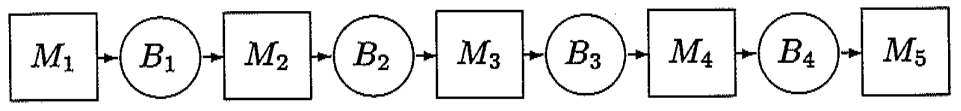
\includegraphics[width=12cm]{transfer_line.png}
\caption{单产品多阶段生产}
\label{fig:transfer_line}
\end{figure}

多阶段生产中的重要制约因素是机器故障。机器故障有两种模式:基于时间的故障模式和基于运作的故障模式。两种模式都是随机的。基于时间的故障模式下,机器故障的发生取决于使用的时间长短,比如材料的强度失效;基于运作的故障模式下,机器故障的发生取决于使用次数或产量,比如刀具失效。

机器即使没有出故障,也不一定能运转,因为还受到上下游库存的限制。如果上游库存不足,导致下游机器停工,我们称下游机器为缺料状态;如果下游库存已满,导致上游机器停工,我们称上游机器为阻塞状态。

缓存区的库存被称为在途库存。在多阶段生产中,在途库存往往是必不可少的,因为它能减少机器故障带来的损失。当一台机器出现故障时,上游的机器可以继续运转,生产的产品进入在途库存;下游机器也能依靠故障机器的在途库存提供原料继续运转。但在途库存也会带来一些问题,Gershwin在书中总结了在途库存的主要缺点:
\begin{enumerate}
\item
在途库存是消耗资金制造出来的,占用了资金却不产生任何效益。
\item
根据Little's Law \cite{little_proof_1961} ,在途库存对提前期有影响。在途库存越多,提前期越长。提前期过长可能导致顾客不满,同时也使得生产中的故障更难以被观察到。在观察到故障之前,故障机器可能已经制造了很多残次品。
\item
零部件在库存期间可能遭受破损、偷窃等损失。库存量越大、时间越长,遭受的损失越大。
\item
储存用的场地和设备会消耗空间和资金。
\end{enumerate}

Gershwin还用马尔科夫模型分析了多阶段生产线在缓存容量上限$N=0$和$N=\infty$的极端情形下的表现,得出了两个重要的结论:
\begin{enumerate}
\item
在$N=0$的情况下,多阶段生产线的运作时间与总时间之比总是随机器数目增加而减小,并且收敛于0。也就是说,如果没有在途库存,当产品需要的生产阶段很多时,生产线的效率将趋近于0。
\item
在$N=\infty$的情况下,多阶段生产线的产能总是取决于最慢的一台机器。也就是说,总体产能只有在瓶颈阶段可能得到优化。
\end{enumerate}

Gershwin指出,用马尔科夫模型研究多阶段生产还存在一些难点。最突出的难点就是状态空间过大。每个机器有2种状态,每个缓存有$N+1$种状态,马尔科夫模型的状态空间就是它们的乘积,即
\[
M = 2^k \prod_{i=0}^{k-1}(N_i+1)
\]
随着阶段数目的增加,状态空间$M$很快就变得非常庞大。

Goyal(1978) \cite{goyal_economic_1978} 考虑需求分布均匀、不允许缺货的多阶段生产,建立了以减少总成本为优化准则的数学模型,用于分析最优的生产批量以及各阶段之间最优的运输批量。

Kimura和Terada(1981)\cite{kimura_design_1981} 分析了多阶段拉动式生产的需求和库存波动是如何逐级传递的,证明了拉动式生产系统比推动式生产系统更能适应需求的波动,并能够防止下游的生产和库存波动向上游逐级扩大。Kimura和Terada所定义的拉动式生产系统需要满足以下运行方式:建立标准的再订货点和订货批量大小;随时了解库存水平和延期订单;连续检查库存水平,一旦某些零部件数量低于再订货点,就立即向上游订货。拉动式生产系统中使用看板来维持运作,流程如图 \ref{fig:pull_system} 所示。

\begin{figure}[htbp]
\centering
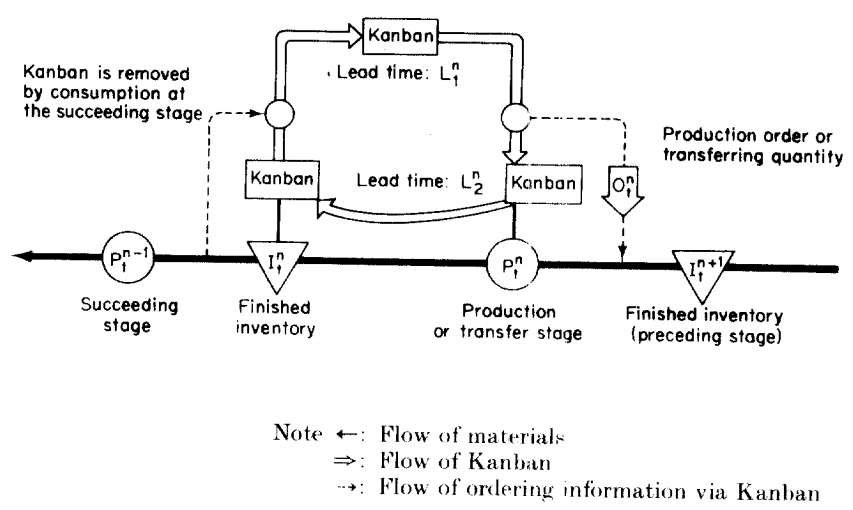
\includegraphics[width=12cm,angle=1,origin=c]{pull_system.png}
\caption{拉动式生产系统流程图}
\label{fig:pull_system}
\end{figure}

研究中使用的推动式生产系统是Tabe等人(1980) \cite{tabe_analysis_1980} 建立的模型,如图 \ref{fig:push_system} 所示。

\begin{figure}[htbp]
\centering
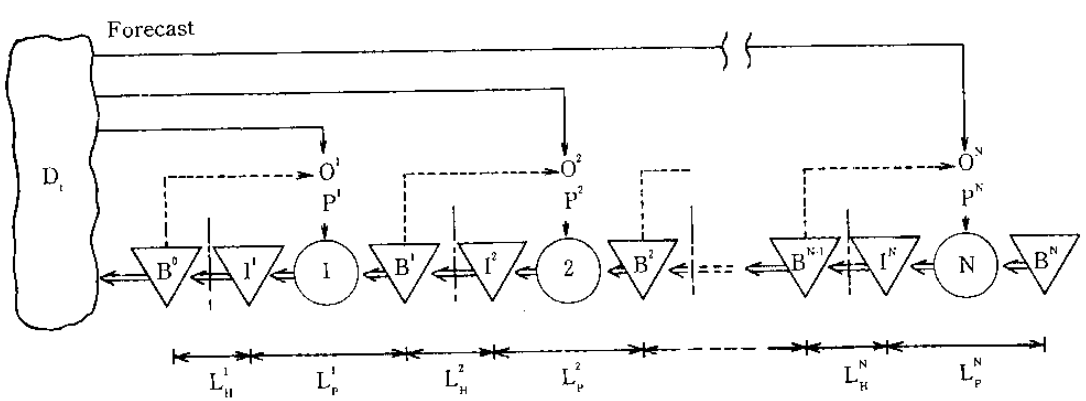
\includegraphics[width=12cm,angle=-1,origin=c]{push_system.png}
\caption{推动式生产系统流程图}
\label{fig:push_system}
\end{figure}

通过数学模型分析和仿真模型实验,Kimura和Terada得到如下结论:
\begin{enumerate}
\item
拉动式生产系统中,单位订货量的大小非常重要。在单位订货量与产量水平相比很小的情况下,拉动式生产中的下游生产波动不会在向上游传递的过程中放大。
\item
推动式生产系统中,生产和库存波动的放大率取决于预测误差。以波动放大率为准则时,推动式系统和拉动式系统之间的抉择取决于预测误差的大小。
\item
拉动式生产系统中另一个影响波动放大率的参数是从看板离开容器到该阶段完成生产的时间差。这个时间差越长,波动放大率越高。
\end{enumerate}

Conway等人(1988) \cite{conway_role_1988} 反对一味追求降低在途库存的做法,全面总结了在途库存在多阶段生产中的意义和作用,并分析各种情况下如何真正改善多阶段生产的绩效。该研究中有以下一些重要的结论:
靠前的几个阶段对整条生产线的产能影响最大,长生产线的绩效比短生产线差得不多;
添加缓存对绩效的提升较大,但增加缓存容量的效果不显著;
在生产线靠中间的位置添加缓存,效果比靠两端的位置好得多;
在未平衡的生产线中添加buffer效果不显著。








\section{风险分担}

已读17篇risk pooling相关文献,待补充文献综述。











\section{延迟差异化}

已读10篇postponement相关文献,待补充文献综述。
\chapter{研究思路}

\section{证明优化潜力存在性}

将成品库存合并前移到在途库存,会造成安全库存的变动。影响这个变动的因素是多方面的:风险分担(risk pooling)使安全库存减少;但在发货之前必须先把在途库存制成成品,相当于增加了提前期,使安全库存增大。

为了证明生产线确实存在优化潜力,我们从极端情况入手,先假设喷涂工序不消耗时间,即忽略库存前移对提前期的影响。如果这种情况下安全库存减少了,那么至少可以认为:新的库存点与成品阶段之间的工序耗时不多的情况下,库存合并前移能减少安全库存。如此即证明了生产线确实存在可优化的潜力。

研究这个问题时,可以首先从最简单的情况入手:假设某注塑件在喷涂阶段分化成两种不同颜色的保险杠成品,并且两种保险杠成品的需求服从独立同分布的正态分布。我们需要证明的是,在这种情况下,如果不保留两种保险杠成品的库存,而是保留喷涂前的注塑件在制品库存,是否能在保持原有服务水平的同时,使得安全库存总量降低。

在此基础上,可以把结论推广到两种不同颜色的保险杠需求独立,但服从不同的正态分布的情况。最后可以推广到多种不同颜色的保险杠需求独立,且服从不同的正态分布的情况。这样,我们就能够证明,当保险杠需求服从独立的正态分布时,将在制品库存保留在分化前的阶段,能够使安全库存总量降低。

正态分布在实际生活中是普遍存在的,并且它拥有很多良好的数学性质,因此我们常常通过对正态分布的研究来作为问题的切入点。但是在讨论生产方面的问题时,我们也常常用泊松过程来模拟一些过程,比如服务的时间、设备的失效或者需求的到达。如果需求的到达是一个泊松过程,则一段时间内的需求就是服从泊松分布的。

可以证明,当泊松分布的参数$\lambda$较大时,可将泊松分布近似处理为正态分布,这样就能把问题转化为刚刚已解决的正态分布的情况。然而在企业的实际生产中,有一些产品的需求量不大,不适合正态近似,因此对泊松分布本身的研究也是必要的。由于泊松分布并不具有正态分布一样良好的数学性质,在对其进行纯数学上的证明遇到困难时,可以考虑用数值模拟的方式进行一些简单的实验。







\section{成品需求相关性的影响}

将不同颜色相同型号的成品库存合并前移,成品之间的相关性必然会影响到方案的效果。因此需要分类讨论成品需求相互独立、需求正相关、需求负相关等情况。
\begin{description}
\item[独立]
成品需求相互独立,意味着一种颜色的保险杠需求量对相同型号另一种颜色的保险杠需求量没有影响。这是最简单的假设,但有时候可能不符合实际情况。
\item[正相关]
某种颜色的保险杠需求变化,可能是由于该车型的市场需求变化。此时该车型的各种颜色需求可能同时变化。也就是说,相同型号不同颜色的保险杠需求可能倾向于同时增大或减小。这是生产实际中可能发生的情况。
\item[负相关]
如果某种车型的市场需求相对稳定,则意味着,一种颜色的需求增长会抑制另一种颜色的需求,表现为相同型号不同颜色的保险杠需求负相关。这也是生产实际中可能发生的情况。
\end{description}

不同的需求相关性会影响库存改进方案的效果。显然,成品需求负相关的情况下,此改进方案的效果将会更加突出。分析成品需求完全正相关和完全负相关的极端情况,能帮助我们明确改进方案的绩效范围,找到改进效果的上下界,从而更好地作出决策。

研究的最后,需要对企业生产线的实际数据进行统计分析,找出不同颜色相同型号的成品需求之间的实际相关性,并针对该结果做具体分析。









\section{提前期变化的影响}

在实际生产中,库存前移会导致供货提前期发生变化。以汽车保险杠的生产为例,假设原定的供货提前期是$T$,喷涂工序所需时间是$t$,在新的库存方案下,由于需要先喷涂再发货,相当于把留给企业的反应时间缩减到了$T-t$,这就对企业的敏捷性和柔性提出了挑战。

显然,当$t$较小时,我们可以忽略它,把问题转化为上面讨论过的情况。但是当$t$值大到不能忽略时,必然会影响到方案的效果,最糟糕的情况下甚至可能使安全库存增大。因此,研究中需要考虑提前期变化对改进方案的影响,希望能找到一定条件下,方案能产生改进效果的提前期临界点,作为决策支持。

研究提前期的影响时仍然可以以正态分布和泊松分布来研究。

正态分布的情况下,可以考虑相同库存总量情况下,改进前后的缺货概率大小。对于改进前后的系统来说,提前期内能够供货的最大量都等于成品库存与提前期内产量之和。以课题背景中提到的汽车保险杠生产为例:
\begin{description}
\item[改进前]
持有各颜色的保险杠成品库存。一旦发现需求过高,成品库存无法满足需求,就需要立即开工生产,先注塑,再喷涂,争取在提前期内生产出足够的数量。
\item[改进后]
不保留成品库存。当需求到来时,从在制品库存中选取相应数量的塑件,经过喷涂后发货;如果发现塑件总量不足以满足需求,则同时启动注塑,以补充塑件在制品库存。
\end{description}
注塑、喷涂各自的生产时间和提前持有的库存总量都会影响两种方案的绩效。此处需要进行更为细致的讨论。

泊松分布的情况下,由于需求是泊松到达,我们可以把问题建模成连续时间的马尔科夫过程,通过求解稳态概率来比较两种方案的缺货概率。由于生产过程不止一个阶段,可能还需要用到Jackson网络。






\section{最优库存策略的探索(待定)}

考虑$(S,s)$库存策略下如何确定最优的$S$和$s$。也可以考虑如何是否只把一部分库存前移能达到最优。






\section{实际生产数据的应用}

在理论研究的结论中代入企业的实际生产数据,检验方案的实际改进效果,为企业提供决策支持。
%本章证明优化潜力的存在性

\chapter{优化潜力存在性}
\label{chapter:优化潜力}

在本章中,我们将忽略相关性和提前期等一切影响因素,单纯从需求的概率分布变化来探究在制品库存前置策略对安全库存的优化作用。






\section{安全库存的制定标准}

安全库存的计算方式是总库存减去需求的期望值。由于本文讨论的所有情况都不涉及需求期望值的变动,因此在比较策略实施前后安全库存的变化时,总库存的减少量与安全库存的减少量始终是等价的。本文后续讨论中不再刻意强调安全库存与总库存的区别,以减少繁琐的数学表达,使数学公式的推导更简洁。

在讨论安全库存时,我们常用的标准有惩罚成本和服务水平。

惩罚成本是企业在缺货时需要付出的成本。合同罚款就是最常见的惩罚成本之一。在汽车配件的生产过程中,配件生产商会和需求方签订合同,当生产商不能按时供货时,就需要承受一笔罚款。惩罚成本能够比较直观地反应缺货带来的损失,体现安全库存的作用。

然而,惩罚成本在使用过程中有一个难以解决的问题:如何准确确定惩罚成本。惩罚成本不仅包括实际的资金损失,还应该考虑其他隐性损失。以汽车配件生产商为例,合同规定的罚款只是表面上的惩罚成本,实际的损失还应该包括企业的声誉损失。汽车行业非常重视精益生产,缺货造成的声誉损失可能使企业丢失更多的潜在订单,甚至失去合作伙伴。这些损失比表面上的罚款更严重,但很难对其进行量化。

因此,如果仅仅使用合同的罚款数额作为惩罚成本,那么分析过程使用的惩罚成本是小于实际损失的。这种情况下,企业做出的决策,会更倾向于承受损失。这是对企业有害的。

本文中,我们将主要使用服务水平作为安全库存的制定标准。这样做的原因不仅包括以上讨论的惩罚成本的缺陷,还有给出更为科学的理由。在接下来的论述中,我们将会证明,如果使用惩罚成本作为安全库存的制定标准,与使用服务水平相比,实质上是等价的。

若只考虑惩罚成本,不考虑库存成本,则企业需要设定一个自己能接受的惩罚成本期望的最大值。我们首先分析惩罚成本的期望。设企业的库存为$K$,惩罚成本为$p$,需求服从分布$P(X=x)=f(x)$,其累积分布为$P(X<x)=F(x)$。则惩罚成本为
\begin{equation}
C(x,K)=\left\{
\begin{aligned}
&0, &x \leq K \\
&p(x-K), &x > K
\end{aligned}
\right.
\label{eq:惩罚成本}
\end{equation}
如果期望存在的话,其对应的期望是
\begin{align}
E[C(x,K)] &= \int_{-\infty}^{+\infty}C(x,K)f(x)\dif x\notag\\
&=\int_K^{+\infty}p(x-K)f(x)\dif x\notag\\
&=p(x-K)F(x)\bigg|_K^{+\infty} - \int_K^{+\infty}pF(x)\dif x\notag\\
&=\lim_{M\to+\infty}\left[p(M-K) - \int_K^MpF(x)\dif x\right]\notag\\
&=\lim_{M\to+\infty}\left[\int_K^Mp\dif x - \int_K^MpF(x)\dif x\right]\notag\\
&=p\int_K^{+\infty}(1-F(x))\dif x
\label{eq:惩罚成本期望}
\end{align}
另一方面,库存为$K$时,对应的服务水平是
\begin{equation}
\eta = \int_{-\infty}^Kf(x)\dif x
\label{eq:服务水平}
\end{equation}

由公式\ref{eq:惩罚成本期望}和\ref{eq:服务水平}可知,惩罚成本期望是随$K$单调递减的,服务水平是随$K$单调递增的。二者可以一一对应,即每个惩罚成本期望值都对应某个特定的服务水平。企业制定自己的惩罚成本期望值,和制定自己的服务水平,是等价的。

使用服务水平来计算安全库存时,不需要考虑库存成本。使用惩罚成本时,可以把库存成本也加入到模型中。接下来我们将证明,加入库存成本之后,惩罚成本与服务水平也是一一对应的。以下推导过程中使用离散的库存量和需求量。

设企业的库存为$K$,需求为$D$,惩罚成本为$p$,库存成本为$h$。则总成本为
\begin{equation}
C(K) = p\max\{D-K,0\} + h(\frac{1}{2}\min\{D,K\}+\max\{K-D,0\})
\label{eq:库存和惩罚成本}
\end{equation}
企业的目标是寻找最优的库存$K$,使得库存成本和惩罚成本之和的期望最小。我们对公式\ref{eq:库存和惩罚成本}中的几个部分分别求期望。
\begin{align}
E(\min\{D,K\}) &= \sum_{i=1}^{\infty}\min\{i,K\}P(D=i) \notag\\
&= \sum_{i=1}^{\infty}\sum_{j=1}^{\min\{i,K\}}P(D=i) \notag\\
&= \sum_{j=1}^K\sum_{i=j}^{\infty}P(D=i) \notag\\
&= \sum_{j=1}^K P(D \geq j) \label{eq:期望1}\\
E(\max\{D-K,0\}) &= -\min\{K-D,0\} \notag\\
&= -(\min\{K,D\}-D) \notag\\
&= D - \sum_{j=1}^K P(D \geq j) \label{eq:期望2}\\
E(\max\{K-D,0\}) &= \sum_{i=1}^{\infty}\max\{K-i,0\}P(D=i) \notag\\
&= \sum_{i=1}^{\infty}\sum_{j=1}^{\max\{K-i,0\}}P(D=i) \notag\\
&= \sum_{j=1}^{K-1}\sum_{i=1}^j P(D=i) \notag\\
&= \sum_{j=1}^{K-1}P(D \leq j) \label{eq:期望3}
\end{align}
将公式\ref{eq:期望1}、\ref{eq:期望2}和\ref{eq:期望3}代入公式\ref{eq:库存和惩罚成本}可得
\begin{equation}
E[C(K)] = pD + (\frac{h}{2}-p)\sum_{j=1}^K P(D \geq j) + h\sum_{j=1}^{K-1} P(D \leq j)
\label{eq:库存和惩罚成本期望}
\end{equation}
考虑库存增加时,总成本的增量
\begin{align}
E[C(K+1)]-E[C(K)] &= (\frac{h}{2}-p)P(D\geq K+1) + hP(D\leq K) \notag\\
&= \frac{h}{2}-p+(\frac{h}{2}+p)P(D\leq K) \label{eq:总成本增量}
\end{align}
公式\ref{eq:总成本增量}是随$K$单调递增的,因此,当$E[C(K+1)]-E[C(K)]$取得0值时,$E[C(K)]$取得最小值。此时有
\begin{equation}
P(D\leq K) = \frac{2p-h}{2p+h}
\label{eq:惩罚成本与服务水平的关系}
\end{equation}

根据服务水平的定义,公式\ref{eq:惩罚成本与服务水平的关系}中的$P(D\leq K)$即是企业的服务水平$\eta$。本文讨论的改进方案仅移动在制品库存在生产线上的位置,不影响库存费用和需求分布。因此,给出任意的惩罚成本,都有一个唯一的服务水平与之对应。

通过以上的讨论,我们已经证明了,以惩罚成本和库存成本来制定安全库存的问题,可以转化为以服务水平来制定安全库存的问题。为了使数学推导更加简洁,本文余下的部分将主要使用服务水平作为安全库存的制定标准。企业可以根据实际情况选取合适的制定方式,且不影响本文中结论的适用性。












\section{两种成品需求独立正态分布}

仍然以汽车保险杠生产为例,假设某种汽车保险杠只有两种颜色,且两种颜色的需求服从独立的正态分布。第一种颜色的保险杠,需求$D_1$服从正态分布$N_1(\mu_1,\sigma_1^2)$;第二种颜色的保险杠,需求$D_2$服从正态分布$N_2(\mu_2,\sigma_2^2)$。企业设定的服务水平为$\eta$。设$z_\eta$是标准正态分布的$\eta$分位数,即$z_\eta$满足
\[
\int_{-\infty}^{z_\eta}\frac{1}{\sqrt{2\pi}}e^{-\frac{x^2}{2}}\dif x = \eta
\]
则此服务水平下,两种成品的库存分别为
\begin{align}
\xi_1 &= \mu_1 + z_\eta\sigma_1 \label{eq:成品库存1}\\
\xi_2 &= \mu_2 + z_\eta\sigma_2 \label{eq:成品库存2}
\end{align}

现在假设我们按照改进策略,取消两种颜色的成品库存,改为保留未喷涂的在制品库存。忽略供货提前期等变化的影响。企业的服务水平仍然为$\eta$。为了满足该服务水平,所需的在制品库存为$\xi$。此时的在制品库存需要同时应对两种颜色的成品需求,因此,对未喷涂的在制品需求为$D=D_1+D_2$。

设$D_1$、$D_2$的联合分布为$f(x_1,x_2)$。因为$D_1$、$D_2$是独立的,所以$f(x_1,x_2)$的概率分布为
\begin{align}
f(x_1,x_2) &= f(x_1)\cdot f(x_2) \notag\\
&= \frac{1}{\sqrt{2\pi}\sigma_1}e^{-\frac{(x_1-\mu_1)^2}{2\sigma_1^2}}\cdot \frac{1}{\sqrt{2\pi}\sigma_2}e^{-\frac{(x_2-\mu_2)^2}{2\sigma_2^2}} \notag\\
&= \frac{1}{2\pi\sigma_1\sigma_2}e^{-\frac{1}{2}\left[\frac{(x_1-\mu_1)^2}{\sigma_1^2}+\frac{(x_2-\mu_2)^2}{\sigma_2^2}\right]}
\label{eq:联合分布}
\end{align}

设$D$、$D_2$的联合分布为$g(y_1,y_2)$。由$y_1=x_1+x_2,y_2=x_2$得$x_1=y_1-y_2,x_2=y_2$。因此,雅可比矩阵为
\[
J = \begin{bmatrix}
\frac{\partial x_1}{\partial y_1} & \frac{\partial x_1}{\partial y_2} \\
\frac{\partial x_2}{\partial y_1} & \frac{\partial x_2}{\partial y_2}
\end{bmatrix} = \begin{bmatrix}
1 & -1 \\
0 & 1
\end{bmatrix}
\]
由此可得$g(y_1,y_2)$的概率分布为
\begin{align}
g(y_1,y_2) &= f(x_1,x_2)\cdot\left|J\right| \notag\\
&= f(y_1-y_2,y_2)\cdot
\begin{vmatrix}
1 & -1 \\
0 & 1
\end{vmatrix} \notag\\
&= \frac{1}{2\pi\sigma_1\sigma_2}e^{-\frac{1}{2}\left[\frac{(y_1-y_2-\mu_1)^2}{\sigma_1^2}+\frac{(y_2-\mu_2)^2}{\sigma_2^2}\right]}
\label{eq:新联合分布}
\end{align}
$g(y_1,y_2)$的边缘分布$h(y_1)$即是在制品需求$D$的概率分布。对$y_2$积分可得
\begin{equation}
h(y_1) = \int_{-\infty}^{+\infty}\frac{1}{2\pi\sigma_1\sigma_2}e^{-\frac{1}{2}\left[\frac{(y_1-y_2-\mu_1)^2}{\sigma_1^2}+\frac{(y_2-\mu_2)^2}{\sigma_2^2}\right]}\dif y_2
\label{eq:求边缘分布}
\end{equation}
令
\[
A = \frac{1}{\sqrt{2\pi(\sigma_1^2+\sigma_2^2)}}e^{-\frac{[y_1-(\mu_1+\mu_2)]^2}{2(\sigma_1^2+\sigma_2^2)}}
\]
则公式\ref{eq:求边缘分布}可变形为
\begin{align}
h(y_1) &= A\int_{-\infty}^{+\infty}\frac{\sqrt{2\pi(\sigma_1^2+\sigma_2^2)}}{2\pi\sigma_1\sigma_2}e^{-\frac{1}{2}\left[\frac{(y_1-y_2-\mu_1)^2}{\sigma_1^2}+\frac{(y_2-\mu_2)^2}{\sigma_2^2}\right]+\frac{[y_1-(\mu_1+\mu_2)]^2}{2(\sigma_1^2+\sigma_2^2)}}\dif y_2 \notag\\
&= A\int_{-\infty}^{+\infty}\frac{\sqrt{\sigma_1^2+\sigma_2^2}}{\sqrt{2\pi}\sigma_1\sigma_2}e^{-\frac{1}{2}\left[\frac{\sqrt{\sigma_1^2+\sigma_2^2}}{\sigma_1\sigma_2}y_2-\left(\frac{\sigma_2}{\sigma_1\sqrt{\sigma_1^2+\sigma_2^2}}(y_1-\mu_1)+\frac{\sigma_1}{\sigma_2\sqrt{\sigma_1^2+\sigma_2^2}}\mu_2\right)\right]^2}\dif y_2
\label{eq:求边缘分布2}
\end{align}
再令
\[
t = \frac{\sqrt{\sigma_1^2+\sigma_2^2}}{\sigma_1\sigma_2}y_2-\left(\frac{\sigma_2}{\sigma_1\sqrt{\sigma_1^2+\sigma_2^2}}(y_1-\mu_1)+\frac{\sigma_1}{\sigma_2\sqrt{\sigma_1^2+\sigma_2^2}}\mu_2\right)
\]
则公式\ref{eq:求边缘分布2}可变形为
\begin{equation}
h(y_1) = A\int_{-\infty}^{+\infty}\frac{1}{\sqrt{2\pi}}e^{-\frac{t^2}{2}}\dif t
\label{eq:求边缘分布3}
\end{equation}
公式\ref{eq:求边缘分布3}的右半部分是标准正态分布的累积概率函数,总累积概率应该为1,即
\[
\int_{-\infty}^{+\infty}\frac{1}{\sqrt{2\pi}}e^{-\frac{t^2}{2}}\dif t = 1
\]
因此得到$h(y_1)=A$,即
\begin{equation}
h(y_1) = \frac{1}{\sqrt{2\pi(\sigma_1^2+\sigma_2^2)}}e^{-\frac{[y_1-(\mu_1+\mu_2)]^2}{2(\sigma_1^2+\sigma_2^2)}}
\label{eq:边缘分布结果}
\end{equation}

由公式\ref{eq:边缘分布结果}可知,在制品的需求$D$服从正态分布$N(\mu_1+\mu_2,\sigma_1^2+\sigma_2^2)$。为了满足服务水平$\eta$,所需的在制品库存为
\begin{equation}
\xi = \mu_1 + \mu_2 + z_\eta\sqrt{\sigma_1^2+\sigma_2^2}
\label{eq:在制品库存}
\end{equation}

至此,我们可以利用公式\ref{eq:成品库存1}、\ref{eq:成品库存2}和\ref{eq:在制品库存}将改进前后的库存总量进行比较
\begin{align}
\xi_1 + \xi_2 - \xi &= \mu_1 + z_\eta\sigma_1 + \mu_2 + z_\eta\sigma_2 - \left(\mu_1 + \mu_2 + z_\eta\sqrt{\sigma_1^2+\sigma_2^2}\right) \notag\\
&= z_\eta\left(\sigma_1+\sigma_2-\sqrt{\sigma_1^2+\sigma_2^2}\right) \notag\\
&> z_\eta\left(\sigma_1+\sigma_2-\sqrt{\sigma_1^2+\sigma_2^2+2\sigma_1\sigma_2}\right) \notag\\
&= z_\eta\left(\sigma_1+\sigma_2-\sqrt{(\sigma_1+\sigma_2)^2}\right) \notag\\
&= 0
\label{eq:改进前后库存比较}
\end{align}
由公式\ref{eq:改进前后库存比较}可知$\xi_1+\xi_2>\xi$,即改进后的在制品库存严格小于改进前的成品库存之和。这个结果说明,当两种不同颜色的成品需求服从独立正态分布时,通过把成品库存合并到在制品库存,能够降低企业的库存总量。



\section{两种以上的成品需求独立正态分布}

现在我们将上述结果进行推广。假设某种汽车保险杠有$N$种颜色($N\geq 2$),并且服从两两相互独立的正态分布。第$i$种颜色的保险杠,需求$D_i$服从正态分布$N_i(\mu_i,\sigma_i^2)$,$i=1,2,\ldots,N$。企业的服务水平仍为$\eta$,其对应的标准正态分布$\eta$分位数仍为$z_\eta$。

为了满足此服务水平,各成品需要保留的库存为
\begin{equation}
\xi_i = \mu_i + z_\eta\sigma_i,\qquad i=1,2,\ldots,N
\label{eq:成品库存i}
\end{equation}

现在假设我们按照改进策略,取消所有颜色的成品库存,改为保留未喷涂的在制品库存。为了满足服务水平$\eta$,所需的在制品库存为$\xi$。此时在制品库存的需求为$D=\sum_{i=1}^ND_i$。前面已证任意两个独立的正态分布之和仍然服从正态分布,由于所有的$D_i$都是相互独立的,因此它们可以连续加和,其结果仍然服从正态分布。所以我们有$D\sim N(\sum_{i=1}^N\mu_i,\sum_{i=1}^N\sigma_i^2)$。进而可以得到在制品库存为
\begin{equation}
\xi = \sum_{i=1}^N\mu_i + z_\eta\sqrt{\sum_{i=1}^N\sigma_i^2}
\label{eq:在制品库存i}
\end{equation}

通过公式\ref{eq:成品库存i}和\ref{eq:在制品库存i}比较改进前后的库存变化
\begin{align}
\sum_{i=1}^N\xi_i - \xi &= \sum_{i=1}^N (\mu_i+z_\eta\sigma_i) - \left(\sum_{i=1}^N\mu_i + z_\eta\sqrt{\sum_{i=1}^N\sigma_i^2}\right) \notag\\
&= z_\eta\left(\sum_{i=1}^N\sigma_i-\sqrt{\sum_{i=1}^N\sigma_i^2}\right) \notag\\
&> z_\eta\left(\sum_{i=1}^N\sigma_i-\sqrt{\sum_{i=1}^N\sigma_i^2+2\sum_{i=1}^{N-1}\sum_{j=i+1}^N\sigma_i\sigma_j}\right) \notag\\
&= z_\eta\left(\sum_{i=1}^N\sigma_i-\sqrt{\left(\sum_{i=1}^N\sigma_i\right)^2}\right) \notag\\
&= 0
\label{eq:改进前后库存比较i}
\end{align}
由公式\ref{eq:改进前后库存比较i}可知$\sum_{i=1}^N\xi_i > \xi$,即改进后的在制品库存严格小于改进前的成品库存。至此,我们已证明,当成品库存服从两两相互独立的正态分布时,通过保留在制品库存能够降低企业的库存总量。








\section{一些参数对改进效果的影响}

前面已经证明了保留在制品库存的改进能够达到降低安全库存的目的,本节将讨论影响改进效果的参数,找出最适宜进行改进的环境。

到目前为止,我们探讨的过程中出现过的参数主要有需求的均值、方差和企业的服务水平。其中,需求的均值决定的是库存中固定的部分而非波动的部分,因此需求均值对于改进效果是没有影响的。我们需要考虑的是需求的方差和企业的服务水平对改进效果的影响。

为了使问题更简单,我们假设只有两种成品参与改进,它们的需求相互独立,且都服从相同的正态分布$N(\mu,\sigma^2)$。由公式\ref{eq:边缘分布结果}可知,改进后的需求服从正态分布$N(2\mu,2\sigma^2)$。企业的服务水平为$\eta$,则改进前的安全库存为$2\cdot z_{\eta}\cdot\sigma$,改进后的安全库存为$z_{\eta}\cdot\sqrt{2}\sigma$。每一个标准差$\sigma$和每一个服务水平$\eta$,都对应着一个改进前后的库存差值$\Delta=2z_{\eta}\sigma-\sqrt{2}z_{\eta}\sigma$。利用计算机程序求出$\sigma\in[0,50]$、$\eta\in(0,1)$的所有对应$\Delta$值,并作图如图\ref{fig:需求波动和服务水平对改进效果的影响}所示。

\begin{figure}[htb]
\centering
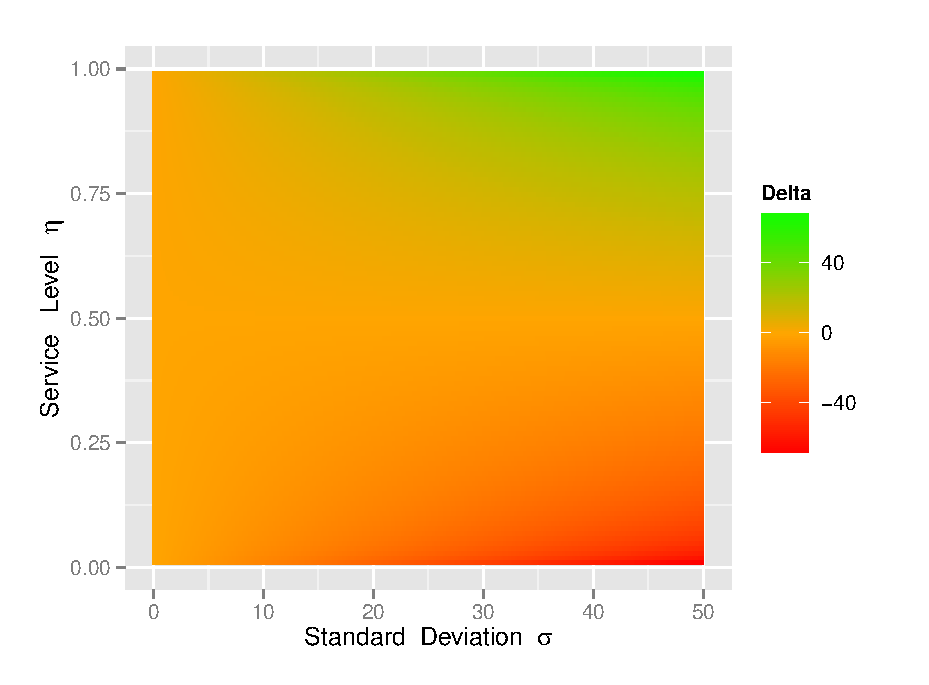
\includegraphics[width=15cm]{normal_effect.eps}
\caption{需求波动和服务水平对改进效果的影响}
\label{fig:需求波动和服务水平对改进效果的影响}
\end{figure}

图\ref{fig:需求波动和服务水平对改进效果的影响}中每个点的位置代表一种$(\sigma,\eta)$组合,每个点的颜色代表该处的$\Delta$值。颜色越绿,代表改进效果越好;颜色越红,代表改进效果越差。

观察图中颜色的分布区域和渐变趋势,可以得到以下结论:
\begin{enumerate}
\item 绿色区域集中在右上角,并向右上方渐变,说明需求波动大、企业服务水平高的环境下,改进效果是最好的,改进策略值得考虑;
\item 红色区域集中在右下角,并向右下方渐变,说明需求波动大、企业服务水平低的环境下,改进效果是最差的,改进之前需要慎重;
\item 需求波动相同的情况下,企业服务水平越高,改进的效果越好;
\item 企业服务水平相同的情况下,需求的波动越强,改进的效果越好。
\end{enumerate}

除此之外还能发现,在$\eta=0.5$处出现了一条“对称轴”,并且该轴两侧的改进效果有正负之别。下一章中,我们将详细讨论这个问题。











%本章探讨改进失效现象

\chapter{改进失效现象}

在第\ref{chapter:优化潜力}章的证明过程中,我们通过添加项的方式对不等式进行放缩,从而证明了$\sum_{i=1}^N\xi_i > \xi$是严格成立的。但是这一推导过程中,我们默认了$z_\eta>0$。由$z_\eta$的定义可知
\[
z_\eta>0 \Longleftrightarrow \eta > 0.5
\]
也就是说,只有当企业设定的服务水平高于50\%时,才能够通过保留在制品库存降低企业库存总量。

当$\eta=0.5$时,有$z_\eta=0$,参考公式\ref{eq:改进前后库存比较i}的推导过程,可知此时$\sum_{i=1}^N\xi_i - \xi = 0$,即改进前后企业的总库存没有发生变化。

当$\eta<0.5$时,有$z_\eta<0$,参考公式\ref{eq:改进前后库存比较i}的推导过程,可以发现此时的不等式放缩方向是相反的,应该得到$\sum_{i=1}^N\xi_i - \xi < 0$,即改进后反而使得企业的总库存增加。

由此可见,当需求服从正态分布时,在某些服务水平下,将成品库存合并前移到在制品库存不仅没有起到改进效果,反而会使总库存增大。我们将这种情况称为改进失效。

本章将结合常用的需求分布函数,详细讨论改进失效现象与需求分布、服务水平等因素的关系。







\section{对称稳定分布的参数与改进失效的关系}

前面的部分主要考虑了需求为正态分布时,改进策略对库存总量的影响。之所以研究正态分布,是因为正态分布确实广泛存在于现实生活中。实际生产中的需求分布可能是各种各样的,甚至可能写不出解析式,但只要是方差有限的独立同分布,根据中心极限定理,在进行叠加的时候总会趋近于正态分布。而正态分布自身叠加仍是正态分布。因此,正态分布就像一个吸引域,从各种分布出发最终都落入正态分布。正态分布下的库存改进效果,也能在很大程度上反应实际的改进效果。

第\ref{chapter:优化潜力}章中已经提到,安全库存等于总库存与需求期望值之差。回顾公式\ref{eq:成品库存i}和\ref{eq:在制品库存i}可知,改进前和改进后的安全库存分别为$z_{\eta}\sum_{i=1}^n\sigma_i$和$z_\eta\sqrt{\sum_{i=1}^n\sigma_i^2}$。为了使考虑的问题更简单,我们假设所有的需求是独立同分布的$N(\mu,\sigma^2)$,则改进前和改进后的安全库存分别为$nz_\eta\sigma$和$\sqrt{n}z_\eta\sigma$。

当$\eta<0.5$的时候,安全库存是负值,这是实际生产中一般不会出现的情况。当$\eta>0.5$时,可以看到,$n$种成品合并之后的安全库存是单个成品安全库存的$\sqrt{n}$倍,而不合并的情况下则是单个成品的$n$倍。此时改进是一定有效果的。

事实上,像正态分布这种“合并后安全库存是单个成品安全库存的$n^{1/\alpha}$倍”的性质,还出现在其他的对称稳定分布中。Feller(2008)\cite{feller_introduction_2008}提到,对称稳定分布有$f_{n,\alpha}(x)=f_\alpha(n^{1/\alpha}x)$的性质。也就是说,$n$个独立同分布的对称稳定分布的随机变量$X$相加,和的概率分布与随机变量$n^{1/\alpha}X$是相同的。而正态分布正是对称稳定分布取$\alpha=2$的一个特例。

稳定分布的概率密度函数为$f(x;\alpha,\beta,c,\mu)$,其中参数$\alpha\in(0,2]$,影响曲线的陡峭程度;$\beta\in[-1,1]$,影响曲线的偏斜程度;$c\in(0,+\infty)$,影响曲线的水平尺度;$\mu\in(-\infty,+\infty)$,影响曲线的水平中心。当$\beta=0$时,即为对称稳定分布。图
\ref{fig:对称稳定分布}展示了$\beta=0,c=1,\mu=0$的对称稳定分布在不同的$\alpha$取值下的图形,其中$\alpha=2$时即为正态分布。

\begin{figure}[htb]
\centering
\includegraphics[width=15cm]{stable.eps}
\caption{不同参数$\alpha$下的对称稳定分布}
\label{fig:对称稳定分布}
\end{figure}

广义中心极限定理指出,$n$个独立同分布的随机变量(方差可以无限)相加,最终会收敛到一个稳定分布。因此,和正态分布一样,稳定分布也广泛存在于实际生活中。Newman(2005)\cite{newman_power_2005}的一系列实证分析证实了这一点。

假设单个成品需求服从对称稳定分布$f(x;\alpha,0,c,\mu)$,则它的安全库存服从对称稳定分布$f(x;\alpha,0,c,0)$。设此需求分布下,满足服务水平$\eta$需要的安全库存为$s$,$n$个成品需要的总安全库存是$ns$。根据(Feller)所述的性质可以推知,改进后需要的安全库存为$n^{1/\alpha}s$。$\eta>0.5$时$s>0$,故改进是否有效就取决于$\alpha$的取值。将改进前后的库存作比较:
\[
\frac{ns}{n^{1/\alpha}s} = n^{1-1/\alpha}
\]
其中$\alpha$的取值范围是$(0,2]$。

当$\alpha\in(1,2]$时,$n^{1-1/\alpha}>1$,改进前的库存大于改进后的库存,改进有效。

当$\alpha\in(0,1]$时,$n^{1-1/\alpha}\leq 1$,改进前的库存不大于改进后的库存,改进无效。









\section{右偏斜的需求分布一定存在改进失效的可能}

对称分布存在一个普遍的缺点——需求可能出现负值,因此我们在实际生产中也常常使用一些其他的分布函数来描述需求的分布。现实的需求不可能为负值,其概率密度函数一般不会有左侧的长尾。因此,需求分布一般都是右偏斜的。Agrawal和Smith(1996)\cite{agrawal_estimating_1996}使用一些实际的需求数据,拟合一些常用的需求分布,包括泊松分布、指数分布、负二项分布等。它们都是右偏斜的分布。

假设有$n$种颜色的成品,其需求$D_i(i=1,2,\ldots,n)$独立同分布且该分布是右偏斜的,累积分布函数都为$F$,均值为$\mu$,方差为$\sigma^2$。将成品库存合并前移到在制品库存后,在制品的总需求为$D_n=\sum_{i=1}^nD_i$,其累积分布函数为$F_n$,均值为$n\mu$,方差为$n\sigma^2$。

设每种颜色的成品库存量为$s$,则对应的服务水平为$\eta=F(s)$。由$F_n$的定义知
\begin{equation}
F_n(ns) = P(D_n<ns) = P\left(\frac{\sum_{i=1}^nD_i}{n}<s\right)
\label{eq:Fn转为均值形式}
\end{equation}

根据中心极限定理,当$n\to\infty$时,$\frac{1}{n}\sum_{i=1}^nD_i$的分布趋近于正态分布$N(\mu,\sigma^2/n)$。设正态分布$N(\mu,\sigma^2/n)$的累积分布函数为$G$。由中心极限定理得
\begin{equation}
\lim_{n\to\infty}P\left(\frac{\sum_{i=1}^nD_i}{n}<s\right) = \lim_{n\to\infty}\Phi\left(\frac{s-\mu}{\sigma/\sqrt{n}}\right) = \lim_{n\to\infty}G(s)
\label{eq:中心极限定理}
\end{equation}
其中$\Phi$为标准正态分布的累积分布函数。由公式\ref{eq:Fn转为均值形式}和\ref{eq:中心极限定理}可知
\begin{equation}
\lim_{n\to\infty}[F_n(ns)-G(s)]=0
\label{eq:Fn与G的极限形式}
\end{equation}

接下来我们将证明,对任何的右偏斜需求分布,一定存在一个区间,当服务水平在此区间内时,就存在改进失效的可能。已知需求$D_i$的分布是右偏的,因此有
\begin{equation}
F(\mu) > 0.5 = \Phi(0) = G(\mu)
\label{eq:右偏斜的性质}
\end{equation}
由$F$和$G$的连续性,至少存在一个$\mu$的领域$[\mu,s_0)$,使得这个区间内的所有库存值$s$都满足
\[
F(s) > G(s),\qquad \forall s\in[\mu,s_0)
\]
令$\delta=F(s)-G(s)>0$。在公式\ref{eq:Fn与G的极限形式}中,根据极限的定义,存在一个正数$N$,使得对任意的$n>N$,都有
\begin{equation}
|F_n(ns)-G(s)| < \delta = F(s) - G(s)
\label{eq:根据极限的定义}
\end{equation}
公式\ref{eq:根据极限的定义}显示,对于任意的$s\in[\mu,s_0)$,都存在一个$N$,使得$n>N$时恒有$F_n(ns)<F(s)$。

我们知道$F(s)$代表需求量小于$s$的概率,即库存量$s$对应的服务水平。反过来,某个服务水平$\eta$也对应着一个库存量,我们将这个对应关系定义为函数$F^{-1}$。函数$F^{-1}$的表达式为
\[
F^{-1}(\eta) = \inf\left\{s\middle|F(s)\geq\eta\right\}
\]
其中$\inf$表示集合的下确界。同理可定义$F_n^{-1}$。

若企业需要满足的服务水平为$\eta$,则改进前和改进后的库存分别为$F^{-1}(\eta)$和$F_n^{-1}(\eta)$。若改进后的在制品库存大于改进前的各颜色成品库存之和,就说明改进失效了。也就是说,改进失效的具体表现是$F_n^{-1}(\eta)>nF^{-1}(\eta)$。下面我们将证明,当$F^{-1}(\eta)\in[\mu,s_0)$时,存在改进失效的可能。

现在假设企业的设定的服务水平为$\eta$,满足$\eta\in[F(\mu),F(s_0))$,则改进前各颜色成品的库存为$s=F^{-1}(\eta)\in[\mu,s_0)$。前面已经证明,对于任意的$s\in[\mu,s_0)$,都存在一个$N$,使得$n>N$时恒有
\begin{equation}
F_n(ns)<F(s)=\eta
\label{eq:改进前后服务水平的关系}
\end{equation}
根据反函数的性质,由于累积分布函数$F$和$F_n$是单调递增的,所以$F^{-1}$和$F_n^{-1}$也是单调递增的。公式\ref{eq:改进前后服务水平的关系}显示$F_n(ns)<\eta$,结合$F_n^{-1}$的单调性可知
\begin{equation}
F_n^{-1}(\eta) > ns
\label{eq:反函数单调性}
\end{equation}
把$s=F^{-1}(\eta)$代入公式\ref{eq:反函数单调性}有
\[
F_n^{-1}(\eta)>nF^{-1}(\eta)
\]
前面已经提到,上式即为改进失效的具体表现。

通过本节的分析,我们证明了,当各颜色成品需求服从独立同分布的任意一种右偏斜分布时,存在一个大于$F^{-1}(\mu)$的服务水平区间,企业的服务水平位于这个区间时,存在改进失效的可能。当服务水平小于$F^{-1}(\mu)$时,安全库存是负值,无需过多讨论。







\section{任何服务水平都存在改进失效的可能}

在上一节的讨论中,我们已经证明,如果需求服从独立同分布的右偏斜分布,则存在一个大于$F^{-1}(\mu)$的服务水平区间,使得这个区间内的服务水平下可能发生改进失效的风险。那么,这个区间是否存在上限?当服务水平远高于$F^{-1}(\mu)$的时候,是否存在某些服务水平,使得在这些服务水平下一定不会发生改进失效?我们以最简单的伯努利分布为例,来研究这个问题。

如果单个产品的需求服从伯努利分布:需求量为$d_1$的概率为$\alpha$,需求量为$d_2$的概率为$1-\alpha$。为了保证需求是右偏的,我们设定$d_1 < d_2$,且$\alpha > 0.5$。

假设有两种颜色的成品,需求相互独立,且都服从上述的伯努利分布。企业的服务水平为$\eta$,则$\eta$和$\alpha$的相对大小会对库存产生影响:当$\eta > \alpha$时,每种成品需要保留的库存为$d_2$,总库存为$2d_2$;当$\eta \leq \alpha$时,每种成品需要保留的库存为$d_1$,总库存为$2d_1$。因此,改进前的服务水平与库存的关系如表\ref{tab:改进前服务水平与库存的关系_伯努利}所示。

\begin{table}[h]
\caption{改进前服务水平与库存的关系}
\label{tab:改进前服务水平与库存的关系_伯努利}
\begin{tabularx}{\textwidth}{YYY}
\toprule
服务水平 & 单个成品库存 & 总库存 \\
\midrule
$\eta > \alpha$ & $d_2$ & $2d_2$ \\
$\eta \leq \alpha$ & $d_1$ & $2d_1$ \\
\bottomrule
\end{tabularx}
\end{table}

现将这两种成品的库存合并保留到在制品库存。首先计算这两种成品需求的联合分布

\begin{table}[h]
\caption{两种成品需求的联合分布}
\label{tab:两种成品需求的联合分布_伯努利}
\begin{tabularx}{\textwidth}{YYY}
\toprule
第一种成品需求 & 第二种成品需求 & 概率 \\
\midrule
$d_1$ & $d_1$ & $\alpha^2$ \\
$d_1$ & $d_2$ & $\alpha(1-\alpha)$ \\
$d_2$ & $d_1$ & $\alpha(1-\alpha)$ \\
$d_2$ & $d_2$ & $(1-\alpha)^2$ \\
\bottomrule
\end{tabularx}
\end{table}


由表\ref{tab:两种成品需求的联合分布_伯努利}可以得到合并后在制品的需求分布,如表\ref{tab:在制品需求分布_伯努利}所示。

\begin{table}[h]
\caption{在制品需求分布}
\label{tab:在制品需求分布_伯努利}
\begin{tabularx}{\textwidth}{YYY}
\toprule
需求量 & 概率 & 累积概率 \\
\midrule
$2d_1$ & $\alpha^2$ & $\alpha^2$ \\
$d_1+d_2$ & $2\alpha(1-\alpha)$ & $2\alpha-\alpha^2$ \\
$2d_2$ & $(1-\alpha)^2$ & $1$ \\
\bottomrule
\end{tabularx}
\end{table}

企业的服务水平仍为$\eta$,根据表\ref{tab:在制品需求分布_伯努利}在制品的需求累积概率分布与$\eta$的相对大小,可以得出需要保留的在制品库存:当$\eta > 2\alpha - \alpha^2$时,在制品需要保留的库存为$2d_2$;当$\alpha^2 < \eta \leq 2\alpha - \alpha^2$时,在制品需要保留的库存为$d_1+d_2$;当$\eta \leq \alpha^2$时,在制品需要保留的库存为$2d_1$。因此,改进后的服务水平与库存的关系如表\ref{tab:改进后服务水平与库存的关系_伯努利}所示。

\begin{table}[h]
\caption{改进后服务水平与库存的关系}
\label{tab:改进后服务水平与库存的关系_伯努利}
\begin{tabularx}{\textwidth}{YYY}
\toprule
服务水平 & 在制品库存 \\
\midrule
$\eta > 2\alpha - \alpha^2$ & $2d_2$ \\
$\alpha^2 < \eta \leq 2\alpha - \alpha^2$ & $d_1+d_2$ \\
$\eta \leq \alpha^2$ & $2d_1$ \\
\bottomrule
\end{tabularx}
\end{table}

对比表\ref{tab:改进前服务水平与库存的关系_伯努利}和表\ref{tab:改进后服务水平与库存的关系_伯努利}可知:当$\eta \leq \alpha^2$时,改进前后的库存都为$2d_1$;当$\alpha^2 < \eta \leq \alpha$时,改进后的库存$2d_2$大于改进前的库存$2d_1$;$\alpha < \eta \leq 2\alpha - \alpha^2$时,改进后的库存$d_1+d_2$小于改进前的库存$2d_2$;当$\eta > 2\alpha - \alpha^2$时,改进前后的库存都为$2d_2$。汇总如表\ref{tab:不同服务水平下改进前后库存对比_伯努利}所示。

\begin{table}[h]
\caption{不同服务水平下改进前后库存对比}
\label{tab:不同服务水平下改进前后库存对比_伯努利}
\begin{tabularx}{\textwidth}{YYY}
\toprule
服务水平 & 改进前库存量 & 改进后库存量 \\
\midrule
$\eta \leq \alpha^2$ & $2d_1$ & $2d_1$ \\
$\alpha^2 < \eta \leq \alpha$ & $2d_1$ & $2d_2$ \\
$\alpha < \eta \leq 2\alpha - \alpha^2$ & $2d_2$ & $d_1+d_2$ \\
$\eta > 2\alpha - \alpha^2$ & $2d_2$ & $2d_2$ \\
\bottomrule
\end{tabularx}
\end{table}

从表\ref{tab:不同服务水平下改进前后库存对比_伯努利}中可以看出,当$\alpha^2 < \eta \leq \alpha$时,一定会发生改进失效。显然,对任意的服务水平$\eta$,一定存在某些$\alpha$,使得$\alpha^2 < \eta \leq \alpha$。因此,任意的服务水平下都能够找到某些右偏斜的伯努利分布,使得改进失效。

上述结论很容易推广到三种以上成品合并库存的情况。假设有$n$种颜色的成品,需求服从独立同分布的伯努利分布,需求量为$d_1$的概率为$\alpha$,需求量为$d_2$的概率为$1-\alpha$,$d_1 < d_2$,$\alpha > 0.5$。易知,当服务水平$\eta \leq \alpha$时,需要保留的单个成品库存量为$d_1$,总库存量为$nd_1$。将它们的库存合并到在制品库存后,在制品的需求服从二项分布,即
\[
P(kd_1+(n-k)d_2) = C_{n}^{k}\alpha^k(1-\alpha)^{n-k}
\]
取$k=n$可知$P(nd_1)=\alpha^n$,因此当服务水平$\eta > \alpha^n$时,需要保留的在制品库存量是大于$nd_1$的。当服务水平满足$\alpha^n < \eta \leq \alpha^n$时,一定发生改进失效。

通过以上讨论我们证明了,将$n$种颜色的成品库存合并为在制品库存时,对于任意的服务水平$\eta$,都可能在某些右偏的需求分布下发生改进失效。因此,企业在做出决策之前不能盲目乐观,必须根据自身的服务水平和实际的需求分布,谨慎地进行模拟和推算,防止发生改进失效。








\section{泊松分布下发生改进失效的区间图示}

在前两节的讨论中,我们从理论上证明了改进失效现象的存在性。但是,对改进失效现象发生的具体范围和如何避免,仍然没有清晰直观的认识。本节中,我们将以实际生产中常用的泊松分布为例,展示改进失效的实际影响和避免改进失效的方法。

为了精确描述库存总量在改进前后的变化,我们首先需要知道改进前后需求分布的变化。设需求$D$服从泊松分布$Po(\lambda)$,则其概率为
\[
P(D=x) = \frac{e^{-\lambda}\lambda^x}{x!},\qquad x\in\mathbb{N}
\]

设企业的服务水平为$\eta$,满足此服务水平所需的库存为$\xi$。则库存$\xi$的表达式为
\begin{equation}
\xi = \inf\left\{\xi\in\mathbb{N}\middle|\sum_{x=0}^{\xi}\frac{e^{-\lambda}\lambda^x}{x!}\geq \eta\right\}
\end{equation}
其中符号$\inf$表示集合的下确界。

设两种颜色的成品需求服从相互独立的泊松分布$Po(\lambda_1)$、$Po(\lambda_2)$。企业的服务水平为$\eta$。则两种成品需要保持的库存$\xi_1$、$\xi_2$分别为
\begin{align}
\xi_1 &= \inf\left\{\xi_1\in\mathbb{N}\middle|\sum_{x=0}^{\xi_1}\frac{e^{-\lambda_1}\lambda_1^x}{k!}\geq \eta\right\} \label{eq:成品库存_泊松1}\\
\xi_2 &= \inf\left\{\xi_2\in\mathbb{N}\middle|\sum_{x=0}^{\xi_2}\frac{e^{-\lambda_2}\lambda_2^x}{k!}\geq \eta\right\} \label{eq:成品库存_泊松2}
\end{align}

现在假设取消两种颜色的成品库存,改为保留共同的在制品库存。企业的服务水平仍然为$\eta$。为了满足该服务水平,所需的在制品库存为$\xi$。此时的在制品库存需要同时应对两种颜色的成品需求,因此,对未喷涂的在制品需求为$D=D_1+D_2$。

设$D_1$、$D_2$的联合分布为$f(x_1,x_2)$。因为$D_1$、$D_2$是独立的,所以$f(x_1,x_2)$的概率分布为
\begin{align}
f(x_1,x_2) &= f(x_1)f(x_2) \notag\\
&= \frac{e^{-\lambda_1}\lambda_1^{x_1}}{x_1!} \cdot \frac{e^{-\lambda_2}\lambda_2^{x_2}}{x_2!} \notag\\
&= \frac{e^{-(\lambda_1+\lambda_2)}\lambda_1^{x_1}\lambda_2^{x_2}}{x_1!x_2!}
\label{eq:联合分布_泊松}
\end{align}

设$D$、$D_2$的联合分布为$g(y_1,y_2)$。由$y_1=x_1+x_2,y_2=x_2$得$x_1=y_1-y_2,x_2=y_2$。与正态分布下的证明过程类似,我们求出雅可比矩阵
\[
J = \begin{bmatrix}
\frac{\partial x_1}{\partial y_1} & \frac{\partial x_1}{\partial y_2} \\
\frac{\partial x_2}{\partial y_1} & \frac{\partial x_2}{\partial y_2}
\end{bmatrix} = \begin{bmatrix}
1 & -1 \\
0 & 1
\end{bmatrix}
\]
由此可得$g(y_1,y_2)$的概率分布为
\begin{align}
g(y_1,y_2) &= f(y_1-y_2,y_2)\cdot\left|J\right| \notag\\
&= \frac{e^{-(\lambda_1+\lambda_2)}\lambda_1^{y_1-y_2}\lambda_2^{y_2}}{(y_1-y_2)!y_2!}
\label{eq:新联合分布_泊松}
\end{align}
然后求边缘分布$h(y_1)$。与前面不同的是,泊松分布的自变量$y_1-y_2\geq 0$,因此有$y_2\leq y_1$。
\begin{align}
h(y_1) &= \sum_{y_2=0}^{y_1}g(y_1,y_2) = \sum_{y_2=0}^{y_1}\frac{e^{-(\lambda_1+\lambda_2)}\lambda_1^{y_1-y_2}\lambda_2^{y_2}}{(y_1-y_2)!y_2!} \notag\\
&= \frac{e^{-(\lambda_1+\lambda_2)}(\lambda_1+\lambda_2)^{y_1}}{y_1!}\sum_{y_2=0}^{y_1}\frac{y_1!}{y_2!(y_1-y_2)!}\left(\frac{\lambda_1}{\lambda_1+\lambda_2}\right)^{y_1-y_2}\left(\frac{\lambda_2}{\lambda_1+\lambda_2}\right)^{y_2}
\label{eq:求边缘分布_泊松}
\end{align}
公式\ref{eq:求边缘分布_泊松}的右半部分是二项分布$B(y_1,\frac{\lambda_2}{\lambda_1+\lambda_2})$的全部累积概率,其和应该为1,即
\[
\sum_{y_2=0}^{y_1}\frac{y_1!}{y_2!(y_1-y_2)!}\left(\frac{\lambda_1}{\lambda_1+\lambda_2}\right)^{y_1-y_2}\left(\frac{\lambda_2}{\lambda_1+\lambda_2}\right)^{y_2} = 1
\]
因此得到边缘分布为
\begin{equation}
h(y_1) = \frac{e^{-(\lambda_1+\lambda_2)}(\lambda_1+\lambda_2)^{y_1}}{y_1!}
\label{eq:边缘分布结果_泊松}
\end{equation}

由公式\ref{eq:边缘分布结果_泊松}可知,在制品的总需求$D$服从泊松分布$Po(\lambda_1+\lambda_2)$。所以应保留的在制品库存为
\begin{equation}
\xi = \inf\left\{\xi\in\mathbb{N}\middle|\sum_{x=0}^{\xi}\frac{e^{-(\lambda_1+\lambda_2)}(\lambda_1+\lambda_2)^x}{x!}\geq \eta\right\}
\label{eq:在制品库存_泊松}
\end{equation}

根据公式\ref{eq:成品库存_泊松1}、\ref{eq:成品库存_泊松2}和\ref{eq:在制品库存_泊松},如果改进前的需求分布服从$Po(\lambda_1)$和$Po(\lambda_2)$,则改进后的需求服从$Po(\lambda_1+\lambda_2)$。据此,我们就可以算出各种情况下改进前后的库存具体数值,从而进行比较。

为了方便作图,我们假设两种成品的需求是独立同分布的,都服从泊松分布$Po(\lambda)$,则改进后的在制品需求服从泊松分布$Po(2\lambda)$。企业的服务水平为$\eta$。$Po^{-1}_{\lambda}(\eta)$表示改进前的每种成品的库存,$Po^{-1}_{2\lambda}(\eta)$表示改进后的在制品总库存。每一个参数$\lambda$和每一个服务水平$\eta$,都对应着一个改进前后的库存差值$\Delta=2Po^{-1}_{\lambda}(\eta)-Po^{-1}_{2\lambda}(\eta)$。利用计算机程序求出$\lambda\in(0,100)$、$\eta\in(0.5,1)$的所有对应$\Delta$值,并作图如图\ref{fig:泊松分布下的改进失效区间图示}所示。

\begin{figure}[htb]
\centering
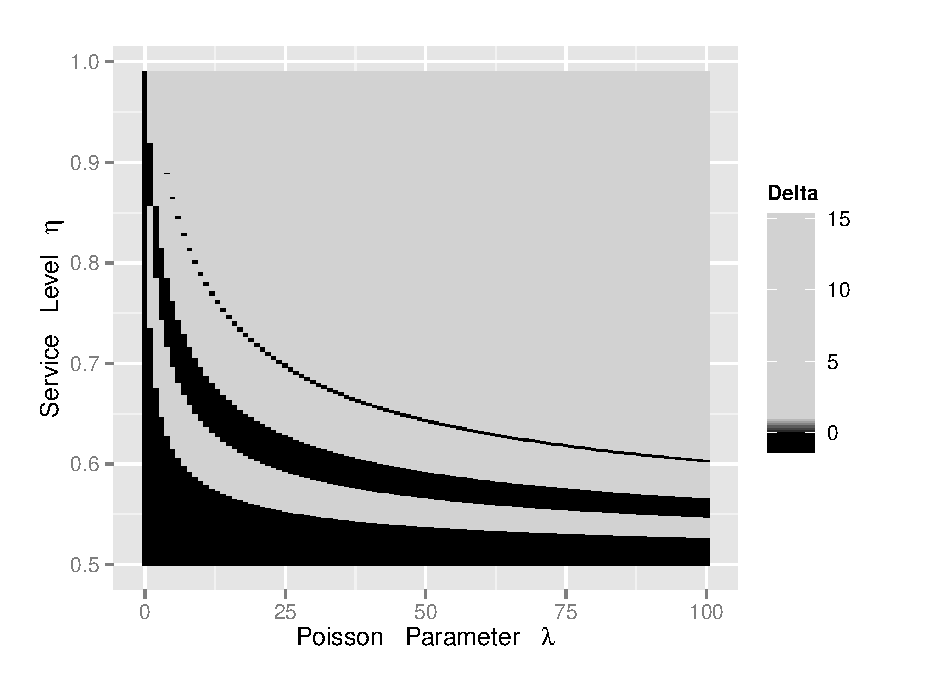
\includegraphics[width=15cm]{ShiXiao.eps}
\caption{泊松分布下的改进失效区间图示}
\label{fig:泊松分布下的改进失效区间图示}
\end{figure}

图\ref{fig:泊松分布下的改进失效区间图示}中每个点的位置代表一种$(\lambda,\eta)$组合,每个点的颜色代表该处的$\Delta$值。如果$\Delta\leq0$,则该点为黑色;如果$\Delta>0$,则该点为浅灰色。因此,图中的黑色区域代表发生改进失效的区域,灰色区域代表改进有效果的区域。

由于泊松分布的离散性,图\ref{fig:泊松分布下的改进失效区间图示}中的黑色区域边缘存在锯齿,甚至是断断续续的。从这幅图形中,我们能够得到很多有效的信息。

首先,它验证了前两节证明的一些论断。作为右偏斜分布的泊松分布,在服务水平大于0.5的某个区间内,确实出现了改进失效的一片区域;另外,当$\lambda\to0$时,黑色区域的延伸趋势也验证了上一节的论断,即不存在“不会发生改进失效的服务水平”。

其次,黑色区域在横轴方向的变化趋势告诉我们,需求量越大,发生改进失效的服务水平区间就越小,也就是说越不容易发生改进失效。当$\lambda$增大到一定程度时,泊松分布会趋近于正态分布。我们已经了解到,正态分布在$\eta>0.5$的时候是不会出现改进失效的。因此,随着$\lambda$的增长,黑色区域会越来越小,最终小到可以忽略的程度。结合上一节中伯努利分布的讨论可以看出,对于右偏斜的需求分布,偏斜程度越大,越可能发生改进失效。

最后,黑色区域在纵轴方向的变化趋势显示,服务水平越高,发生改进失效的区域越少。也就是说,这样的改进方法对于服务水平高的企业是有利的。虽然理论上不存在“不会发生改进失效的服务水平”,但是如果已经知道了需求的参数$\lambda$的一个确定的下限,就能够指出一个对应的服务水平的安全线,使得服务水平高于这个安全线时不可能发生改进失效。












\subsection{第二类服务水平与改进失效}

到目前为止,我们在提到服务水平时,都是指第一类服务水平,即得到满足的订单数占总订单数的比例。在实际生产中,也有一些企业采用第二类服务水平作为库存的制定标准。第二类服务水平是指得到满足的需求量占总需求量的比例。如果库存不足以满足需求,就从需求中减去现有的全部库存,剩余的量才作为未满足的需求量。下面我们将证明,如果改进前后都以相同的第二类服务水平作为制定库存的标准,则不可能发生改进失效。

我们知道,发生改进失效的判定标准是“服务水平不变的情况下,改进后的总库存大于改进前的总库存”。事实上,因为服务水平是随库存增加而单调增加的,因此上述判定标准等价于“总库存不变的情况下,改进后的服务水平低于改进前的服务水平”。所以,如果保持改进前后库存总量不变,只需证明改进后的第二类服务水平不可能低于改进前的第二类服务水平即可。

设两种成品的需求$D_1$、$D_2$相互独立,概率密度函数分别为$f_1(x_1)$和$f_2(x_2)$。企业的服务水平(第二类服务水平)为$\eta$。该服务水平下,两种成品的库存分别为$\xi_1$和$\xi_2$。根据第二类服务水平的定义,得到满足的需求量与总需求量之比的期望值为第二类服务水平。两种成品得到满足的需求量分别为$\min(x_1,\xi_1)$和$\min(x_2,\xi_2)$,因此有
\[
\eta = \int_{-\infty}^{+\infty}\frac{\min(x_1,\xi_1)}{x_1}f(x_1)\dif x_1 = \int_{-\infty}^{+\infty}\frac{\min(x_2,\xi_2)}{x_2}f(x_2)\dif x_2
\]

考虑两种成品需求的联合分布$f(x_1,x_2)$。由于需求是相互独立的,因此有$f(x_1,x_2)=f(x_1)f(x_2)$。将两种成品看做一个整体,则得到满足的需求量为$\min(x_1,\xi_1)+\min(x_2,\xi_2)$,总需求量为$x_1+x_2$。因为它们各自的服务水平都是$\eta$,所以综合服务水平也是$\eta$。因此有
\begin{equation}
\eta = \int_{-\infty}^{+\infty}\int_{-\infty}^{+\infty}\frac{\min(x_1,\xi_1)+\min(x_2,\xi_2)}{x_1+x_2}f(x_1)f(x_2)\dif x_1 \dif x_2
\label{eq:合并前第二类服务水平}
\end{equation}

现将两种成品库存合并到在制品库存,保持总量不变,即合并后的库存为$\xi=\xi_1+\xi_2$。合并后的服务水平为$\eta'$。合并后的总需求量为$x_1+x_2$,其中得到满足的需求量为$\min(x_1+x_2,\xi_1+\xi_2)$,因此合并后的服务水平为
\begin{equation}
\eta' = \int_{-\infty}^{+\infty}\int_{-\infty}^{+\infty}\frac{\min(x_1+x_2,\xi_1+\xi_2)}{x_1+x_2}f(x_1)f(x_2)\dif x_1 \dif x_2
\label{eq:合并后第二类服务水平}
\end{equation}

为了比较$\eta$和$\eta'$的大小,我们先证明$\min(x_1,\xi_1)+\min(x_2,\xi_2)\leq\min(x_1+x_2,\xi_1+\xi_2)$。设$m_1=\min(x_1,\xi_1)$,$m_2=\min(x_2,\xi_2)$,则有$m_1\leq x_1$,$m_1\leq\xi_1$,$m_2\leq x_2$,$m_2\leq\xi_2$。因此$x_1+x_2\geq m_1+m_2$,$\xi_1+\xi_2\geq m_1+m_2$。由此可证
\begin{align}
\min(x_1+x_2,\xi_1+\xi_2) &\geq \min(m_1+m_2,m_1+m_2) \notag\\
&= m_1+m_2 \notag\\
&= \min(x_1,\xi_1)+\min(x_2,\xi_2)
\label{eq:局部放缩_第二类服务水平}
\end{align}

将不等式\ref{eq:局部放缩_第二类服务水平}代入公式\ref{eq:合并前第二类服务水平}和\ref{eq:合并后第二类服务水平}中,就能比较$\eta$和$\eta'$的大小,具体过程如下:

\begin{align}
\eta' &= \int_{-\infty}^{+\infty}\int_{-\infty}^{+\infty}\frac{\min(x_1+x_2,\xi_1+\xi_2)}{x_1+x_2}f(x_1)f(x_2)\dif x_1 \dif x_2 \notag\\
&\geq \int_{-\infty}^{+\infty}\int_{-\infty}^{+\infty}\frac{\min(x_1,\xi_1)+\min(x_2,\xi_2)}{x_1+x_2}f(x_1)f(x_2)\dif x_1 \dif x_2 \notag\\
&= \eta
\label{eq:比较改进前后第二类服务水平}
\end{align}

由公式\ref{eq:比较改进前后第二类服务水平}可知,总库存保持不变的情况下,改进后的第二类服务水平不低于改进前的第二类服务水平。因此,保持第二类服务水平不变的情况下,改进后的库存不会大于改进前的库存。

至此,我们证明了本小节开头提出的观点,即“如果改进前后都以相同的第二类服务水平作为制定库存的标准,则不可能发生改进失效”。因此,对于使用第二类服务水平作为库存制定标准的企业来说,这样的改进是值得考虑的。












\section{避免改进失效}

通过本章的探讨,我们初步了解了改进失效现象的影响因素和具体表现。作为对本章的一个总结,我们在此简单归纳各种参数对改进失效的影响,作为企业改进前需要考虑的因素:

\begin{enumerate}
\item 如果需求服从正态分布,只需保证企业的服务水平大于0.5,即可避免改进失效;
\item 如果需求服从对称稳定分布,需要保证决定分布陡峭程度的参数$\alpha$的值在$(1,2]$区间内,才能避免改进失效;
\item 如果需求服从右偏斜的分布,需要关注需求分布的偏斜程度和企业的服务水平。分布的偏斜程度越大,,越可能发生改进失效;企业的服务水平越低,越可能发生改进失效。
\end{enumerate}

总而言之,企业做出改进决策之前,首先需要考虑的就是需求分布的特点,其次需要检查自身的服务水平在这个需求分布下有无改进失效的可能。






















%本章探讨成品需求相关性对改进效果的影响

\chapter{需求相关性对改进效果的影响}

在之前的讨论中,我们总是假设成品的需求分布是相互独立的。事实上,现实中的两种相似成品的需求往往存在一些相关性。本章将讨论成品需求之间的相关性对改进方案的效果的影响。






\section{需求服从二维正态分布的情况}

为了构造相关系数为$\rho$的两个正态分布的需求变量,我们假设两种颜色的成品需求$(D_1,D_2)$服从二维正态分布$N(\mu_1,\mu_2,\sigma_1^2,\sigma_2^2,\rho)$,则它们的联合分布为
\begin{equation}
f(x_1,x_2) = \frac{1}{2\pi\sigma_1\sigma_2\sqrt{1-\rho^2}}e^{-\frac{1}{2(1-\rho^2)}\left[\frac{(x_1-\mu_1)^2}{\sigma_1^2}+\frac{(x_2-\mu_2)^2}{\sigma_2^2}-\frac{2\rho(x_1-\mu_1)(x_2-\mu_2)}{\sigma_1\sigma_2}\right]}
\label{eq:二维正态分布概率密度}
\end{equation}
对$x_2$积分,可以得到$D_1$的边缘分布
\begin{equation}
f_1(x_1) = \int_{-\infty}^{+\infty}\frac{1}{2\pi\sigma_1\sigma_2\sqrt{1-\rho^2}}e^{-\frac{1}{2(1-\rho^2)}\left[\frac{(x_1-\mu_1)^2}{\sigma_1^2}+\frac{(x_2-\mu_2)^2}{\sigma_2^2}-\frac{2\rho(x_1-\mu_1)(x_2-\mu_2)}{\sigma_1\sigma_2}\right]}\dif x_2
\label{eq:二维边缘分布推导}
\end{equation}
令
\[
A = \frac{1}{\sqrt{2\pi}\sigma_1}e^{-\frac{(x_1-\mu_1)^2}{2\sigma_1^2}}
\]
则公式\ref{eq:二维边缘分布推导}可变形为
\begin{equation}
f_1(x_1) = A\int_{-\infty}^{+\infty}\frac{1}{\sqrt{2\pi(1-\rho^2)}\sigma_2}e^{-\frac{1}{2}\left[\frac{\sigma_1(x_2-\mu_2)-\rho\sigma_2(x_1-\mu_1)}{\sqrt{1-\rho^2}\sigma_1\sigma_2}\right]^2}\dif x_2
\label{eq:二维边缘分布变形}
\end{equation}
再令
\[
t = \frac{\sigma_1(x_2-\mu_2)-\rho\sigma_2(x_1-\mu_1)}{\sqrt{1-\rho^2}\sigma_1\sigma_2}
\]
则公式\ref{eq:二维边缘分布变形}可变形为
\begin{equation}
f_1(x_1) = A\int_{-\infty}^{+\infty}\frac{1}{\sqrt{2\pi}}e^{-\frac{t^2}{2}}\dif t
\label{eq:二维边缘分布变形2}
\end{equation}
公式\ref{eq:二维边缘分布变形2}的有半部分是标准正态分布的累积概率,总累积概率应为1,即
\[
\int_{-\infty}^{+\infty}\frac{1}{\sqrt{2\pi}}e^{-\frac{t^2}{2}}\dif t = 1
\]
因此得到$f_1(x_1)=A$,即
\begin{equation}
f_1(x_1) = \frac{1}{\sqrt{2\pi}\sigma_1}e^{-\frac{(x_1-\mu_1)^2}{2\sigma_1^2}}
\label{eq:二维边缘分布1}
\end{equation}
同理有
\begin{equation}
f_2(x_2) = \frac{1}{\sqrt{2\pi}\sigma_2}e^{-\frac{(x_2-\mu_2)^2}{2\sigma_2^2}}
\label{eq:二维边缘分布2}
\end{equation}

公式\ref{eq:二维边缘分布1}和\ref{eq:二维边缘分布2}表明,当需求$D_1$、$D_2$服从二维正态分布$N(\mu_1,\mu_2,\sigma_1^2,\sigma_2^2,\rho)$时,它们分别服从一维正态分布$N(\mu_1,\sigma_1^2)$和$N(\mu_2,\sigma_2^2)$。下面证明,正态分布的两个变量$D_1$、$D_2$之间的相关系数为$\rho$。

由相关系数的定义可知
\begin{align}
\operatorname{Corr}(D_1,D_2) &= \int_{-\infty}^{+\infty}\int_{-\infty}^{+\infty}\frac{(x_1-\mu_1)(x_2-\mu_2)}{\sigma_1\sigma_2}f(x_1,x_2)\dif x_1\dif x_2 \notag\\
&= \int_{-\infty}^{+\infty}\frac{x_2-\mu_2}{\sigma_2}\int_{-\infty}^{+\infty}\frac{x_1-\mu_1}{\sigma_1}f(x_1,x_2)\dif x_1\dif x_2
\label{eq:相关系数定义}
\end{align}
与公式\ref{eq:二维边缘分布变形}类似,令
\[
t = \frac{\sigma_2(x_1-\mu_1)-\rho\sigma_1(x_2-\mu_2)}{\sqrt{1-\rho^2}\sigma_1\sigma_2}
\]
则公式\ref{eq:相关系数定义}变形为
\begin{equation}
\operatorname{Corr}(D_1,D_2) = \int_{-\infty}^{+\infty}\frac{x_2-\mu_2}{\sigma_2}\int_{-\infty}^{+\infty}\frac{e^{-\frac{(x_2-\mu_2)^2}{2\sigma_2^2}}}{2\pi\sigma_2}\left(t\sqrt{1-\rho^2}+\frac{\rho(x_2-\mu_2)}{\sigma_2}\right)e^{-\frac{t^2}{2}}\dif t\dif x_2
\label{eq:相关系数变形}
\end{equation}
易知
\[
\int_{-\infty}^{+\infty}te^{-\frac{t^2}{2}} = 0
\]
且
\[
\int_{-\infty}^{+\infty}e^{-\frac{t^2}{2}} = \sqrt{2\pi}
\]
因此公式\ref{eq:相关系数变形}可得
\begin{align}
\operatorname{Corr}(D_1,D_2) &= \int_{-\infty}^{+\infty}\frac{x_2-\mu_2}{\sigma_2}\left[\frac{\rho(x_2-\mu_2)}{\sqrt{2\pi}\sigma_2^2}\right]\dif x_2 \notag\\
&= \frac{\rho}{\sqrt{2\pi}}\int_{-\infty}^{+\infty}\left(\frac{x_2-\mu_2}{\sigma_2}\right)^2e^{-\frac{1}{2}\left(\frac{x_2-\mu_2}{\sigma_2}\right)^2}\dif \left(\frac{x_2-\mu_2}{\sigma_2}\right)
\label{eq:相关系数变形2}
\end{align}
令
\[
w = \frac{x_2-\mu_2}{\sigma_2}
\]
则公式\ref{eq:相关系数变形2}可变形为
\begin{align}
\operatorname{Corr}(D_1,D_2) &= \frac{\rho}{\sqrt{2\pi}}\int_{-\infty}^{+\infty}w^2e^{-\frac{w^2}{2}}\dif w \notag\\
&= -\frac{\rho}{\sqrt{2\pi}}\int_{-\infty}^{+\infty}w\dif \left(e^{-\frac{w^2}{2}}\right) \notag\\
&= -\frac{\rho}{\sqrt{2\pi}}\left[\left.we^{-\frac{w^2}{2}}\right|_{-\infty}^{+\infty}-\int_{-\infty}^{+\infty}e^{-\frac{w^2}{2}}\dif w\right] \notag\\
&= -\frac{\rho}{\sqrt{2\pi}}\left(0-\sqrt{2\pi}\right) \notag\\
&= \rho
\label{eq:相关系数结果}
\end{align}

至此,我们已构造出两个相关性为$\rho$的需求变量$D_1$和$D_2$,它们各自服从正态分布$N(\mu_1,\sigma_1^2)$和$N(\mu_2,\sigma_2^2)$,并且知道它们的联合分布服从二维正态分布$N(\mu_1,\mu_2,\sigma_1^2,\sigma_2^2,\rho)$。

设企业的服务水平为$\eta$,对应的标准正态分布分位数为$z_\eta$。则两种颜色的成品需要保留的库存$\xi_1$、$\xi_2$分别为
\begin{align}
\xi_1 = \mu_1 + z_\eta\sigma_1 \label{eq:成品库存1_相关性}\\
\xi_2 = \mu_2 + z_\eta\sigma_2 \label{eq:成品库存2_相关性}
\end{align}

现在假设我们按照改进策略,取消两种颜色的成品库存,改为保留未喷涂的在制品库存。忽略供货提前期等变化的影响。企业的服务水平仍然为$\eta$。为了满足该服务水平,所需的在制品库存为$\xi$。此时的在制品库存需要同时应对两种颜色的成品需求,因此,对未喷涂的在制品需求为$D=D_1+D_2$。设$D$、$D_2$的联合分布为$g(y_1,y_2)$。由$y_1=x_1+x_2,y_2=x_2$得$x_1=y_1-y_2,x_2=y_2$。因此,雅可比矩阵为
\[
J = \begin{bmatrix}
\frac{\partial x_1}{\partial y_1} & \frac{\partial x_1}{\partial y_2} \\
\frac{\partial x_2}{\partial y_1} & \frac{\partial x_2}{\partial y_2}
\end{bmatrix} = \begin{bmatrix}
1 & -1 \\
0 & 1
\end{bmatrix}
\]
由此可得$g(y_1,y_2)$的概率分布为
\begin{align}
g(y_1,y_2) &= f(x_1,x_2)\cdot\left|J\right| \notag\\
&= f(y_1-y_2,y_2)\cdot
\begin{vmatrix}
1 & -1 \\
0 & 1
\end{vmatrix} \notag\\
&= \frac{1}{2\pi\sigma_1\sigma_2\sqrt{1-\rho^2}}e^{-\frac{1}{2(1-\rho^2)}\left[\frac{(y_1-y_2-\mu_1)^2}{\sigma_1^2}+\frac{(y_2-\mu_2)^2}{\sigma_2^2}-\frac{2\rho(y_1-y_2-\mu_1)(y_2-\mu_2)}{\sigma_1\sigma_2}\right]}
\label{eq:新联合分布_二维正态}
\end{align}
$g(y_1,y_2)$的边缘分布$h(y_1)$即是在制品需求$D$的概率分布。对$y_2$积分可得
\begin{equation}
h(y_1) = \int_{-\infty}^{+\infty}\frac{1}{2\pi\sigma_1\sigma_2\sqrt{1-\rho^2}}e^{-\frac{1}{2(1-\rho^2)}\left[\frac{(y_1-y_2-\mu_1)^2}{\sigma_1^2}+\frac{(y_2-\mu_2)^2}{\sigma_2^2}-\frac{2\rho(y_1-y_2-\mu_1)(y_2-\mu_2)}{\sigma_1\sigma_2}\right]}\dif y_2
\label{eq:求边缘分布_二维正态}
\end{equation}
令
\[
A = \frac{1}{\sqrt{2\pi(\sigma_1^2+\sigma_2^2+2\rho\sigma_1\sigma_2)}}e^{-\frac{[y_1-(\mu_1+\mu_2)]^2}{2(\sigma_1^2+\sigma_2^2+2\rho\sigma_1\sigma_2)}}
\]
则公式\ref{eq:求边缘分布_二维正态}可变形为
\begin{equation}
h(y_1) = A\int_{-\infty}^{+\infty}\frac{\sqrt{2\pi(\sigma_1^2+\sigma_2^2+2\rho\sigma_1\sigma_2)}}{2\pi\sigma_1\sigma_2\sqrt{1-\rho^2}}e^{-\frac{\sigma_1^2+\sigma_2^2+2\rho\sigma_1\sigma_2}{2\sigma_1^2\sigma_2^2(1-\rho^2)}\left[y_2-\frac{(y_1-\mu_1)\sigma_2^2+\mu_2\sigma_1^2+\rho\sigma_1\sigma_2y_1}{\sigma_1^2+\sigma_2^2+2\rho\sigma_1\sigma_2}\right]^2}\dif y_2
\label{eq:求边缘分布2_二维正态}
\end{equation}
再令
\[
t = \sqrt{\frac{\sigma_1^2+\sigma_2^2+2\rho\sigma_1\sigma_2}{\sigma_1^2\sigma_2^2(1-\rho^2)}}\left[y_2-\frac{(y_1-\mu_1)\sigma_2^2+\mu_2\sigma_1^2+\rho\sigma_1\sigma_2y_1}{\sigma_1^2+\sigma_2^2+2\rho\sigma_1\sigma_2}\right]
\]
则公式\ref{eq:求边缘分布2_二维正态}可变形为
\begin{equation}
h(y_1) = A\int_{-\infty}^{+\infty}\frac{1}{\sqrt{2\pi}}e^{-\frac{t^2}{2}}\dif t
\label{eq:求边缘分布3_二维正态}
\end{equation}
公式\ref{eq:求边缘分布3_二维正态}的右半部分是标准正态分布的累积概率函数,总累积概率应该为1,因此得到$h(y_1)=A$,即
\begin{equation}
h(y_1) = \frac{1}{\sqrt{2\pi(\sigma_1^2+\sigma_2^2+2\rho\sigma_1\sigma_2)}}e^{-\frac{[y_1-(\mu_1+\mu_2)]^2}{2(\sigma_1^2+\sigma_2^2+2\rho\sigma_1\sigma_2)}}
\label{eq:边缘分布结果_二维正态}
\end{equation}

由以上推导可知,在制品需求$D$服从正态分布$N(\mu,\sigma^2)$,其中$\mu=\mu_1+\mu_2$,$\sigma^2=\sigma_1^2+\sigma_2^2+2\rho\sigma_1\sigma_2$。因此,需要保留的在制品库存$\xi$为
\begin{equation}
\xi = \mu + z_\alpha\sigma = \mu_1 + \mu_2 + z_\alpha\sqrt{\sigma_1^2+\sigma_2^2+2\rho\sigma_1\sigma_2}
\label{eq:在制品库存_相关性}
\end{equation}
根据公式\ref{eq:成品库存1_相关性}、\ref{eq:成品库存2_相关性}和\ref{eq:在制品库存_相关性},可以比较改进前后的库存变化。
\begin{align}
\xi_1+\xi_2-\xi &= \mu_1 + z_\alpha\sigma_1 + \mu_2 + z_\alpha\sigma_2 - \left(\mu_1 + \mu_2 + z_\alpha\sqrt{\sigma_1^2+\sigma_2^2+2\rho\sigma_1\sigma_2}\right) \notag\\
&= z_\alpha \left(\sigma_1+\sigma_2-\sqrt{\sigma_1^2+\sigma_2^2+2\rho\sigma_1\sigma_2}\right)
\label{eq:改进前后库存比较_相关性}
\end{align}
我们知道$\sigma_1>0$,$\sigma_2>0$以及$|\rho| \leq 1$,因此有
\begin{equation}
\sqrt{\sigma_1^2+\sigma_2^2+2\rho\sigma_1\sigma_2} \leq \sqrt{\sigma_1^2+\sigma_2^2+2\sigma_1\sigma_2} = \sigma_1+\sigma_2
\label{eq:相关系数放缩}
\end{equation}
将公式\ref{eq:相关系数放缩}代入公式\ref{eq:改进前后库存比较_相关性},得
\begin{equation}
\xi_1+\xi_2-\xi \geq z_\alpha \left[\sigma_1+\sigma_2-(\sigma_1+\sigma_2)\right] = 0
\label{eq:改进前后库存比较结果_相关性}
\end{equation}

公式\ref{eq:改进前后库存比较结果_相关性}的结果表明,对于需求有相关性、服从二维正态分布的两种成品,如果取消成品库存,改为保留共同的在制品库存,在相同的服务水平下,改进后的在制品库存不会比改进前的两种成品库存之和更大。







\section{需求服从多维正态分布的情况}

现在我们将上述结果进行推广。假设某成品有$N$种颜色($N\geq 2$),它们的需求服从多维正态分布,且两两之间的相关系数为$\rho_{ij}$。则每种颜色的库存为
\begin{equation}
\xi_i = \mu_i + z_\alpha\sigma_i,\qquad i=1,2,\ldots,N
\label{eq:成品库存i_相关性}
\end{equation}

假设取消全部成品库存,改为保留共同的在制品库存,则在制品库存$\xi$应为
\begin{equation}
\xi = \sum_{i=1}^N\mu_i + z_\alpha\sqrt{\sum_{i=0}^N\sigma_i^2 + 2\sum_{i=1}^{N-1}\sum_{j=i+1}^N\rho_{ij}\sigma_i\sigma_j}
\label{eq:在制品库存i_相关性}
\end{equation}

根据公式\ref{eq:成品库存i_相关性}和\ref{eq:在制品库存i_相关性}作比较
\begin{align}
\sum_{i=1}^N\xi_i - \xi &= \sum_{i=1}^N(\mu_i+z_\alpha\sigma_i) - \left(\sum_{i=1}^N\mu_i + z_\alpha\sqrt{\sum_{i=0}^N\sigma_i^2 + 2\sum_{i=1}^{N-1}\sum_{j=i+1}^N\rho_{ij}\sigma_i\sigma_j}\right) \notag\\
&= z_\alpha\left(\sum_{i=1}^N\sigma_i-\sqrt{\sum_{i=0}^N\sigma_i^2 + 2\sum_{i=1}^{N-1}\sum_{j=i+1}^N\rho_{ij}\sigma_i\sigma_j}\right) \notag\\
&\geq z_\alpha\left(\sum_{i=1}^N\sigma_i-\sqrt{\sum_{i=0}^N\sigma_i^2 + 2\sum_{i=1}^{N-1}\sum_{j=i+1}^N\sigma_i\sigma_j}\right) \notag\\
& = 0
\label{eq:改进前后库存对比i_相关性}
\end{align}

公式\ref{eq:改进前后库存对比i_相关性}表明,对于两种以上颜色、需求具有相关性的成品,改进后的在制品库存不会比改进前的各颜色成品库存之和更大。






\section{极端情况的讨论}

公式\ref{eq:在制品库存i_相关性}中,$\rho_{ij}$的取值范围是$[-1,1]$。容易发现,在其他参数不变的情况下,当所有的$\rho_{ij}$都同时满足$\rho_{ij}=-1$时,在制品库存$\xi$取得最小值;当所有的$\rho_{ij}$都同时满足$\rho_{ij}=1$时,在制品库存$\xi$取得最大值。

$\rho_{ij}=-1$时,各种颜色的成品需求都是完全负相关的。一种颜色的成品需求增加,就会抑制其他颜色的需求。这种情况主要发生在需求总量稳定、需求偏好不确定的条件下。在制品库存$\xi$取得最小值,说明此时采取保留在制品库存而不是成品库存,优化的收益最大。这与我们的生活经验是相符的。比如全校毕业生征订毕业衫,总需求量几乎是确定的,每个人一般只订一件,且每个人偏好的颜色不同。此时,提前给每种颜色的毕业衫印制足量的库存显然是不妥的,一般会采用先收集订单再印制的方式。

$\rho_{ij}=1$时,各种颜色成品需求都是完全正相关的。一种颜色的成品需求增加,会导致其他颜色的需求同步增加。在制品库存$\xi$取得最大值,说明此事采取保留在制品库存的策略,收益最小。事实上,$\rho_{ij}=1$时,公式\ref{eq:改进前后库存对比i_相关性}中的等号是成立的,即$\sum_{i=1}^N\xi_i - \xi = 0$。换句话说,此时采取保留在制品库存的改进措施毫无效果。

其他情况下,不论各成品的需求是正相关还是负相关,只要不是完全正相关($\rho_{ij}=1$),都能从保留在制品库存的策略中获得收益。并且,与需求独立的情况相比,负相关时的收益更大,正相关时的收益更小。这是企业在做出改进决策之前需要考虑的重要因素。









\section{需求相关性实例}

本文是以汽车行业为课题背景的,

















%本章研究backorder对改进效果的影响

\chapter{Backorder对改进效果的影响}

作为供应商,如果不能按时交货,有时需要将订单记下,尽快补货,并且承受一定的惩罚。这种订单称为backorder。本章中,我们将讨论backorder对我们的方案改进效果的影响。




\section{考虑Backorder成本的任意更新过程}

以汽车保险杠的生产线为例,为了使讨论简化,我们假设注塑环节需要的时间远大于喷涂环节,从而忽略喷涂环节的生产时间。也就是说,改进前后相比,单件产品的生产时间是不变的。

假设有N种颜色的成品,每种产品的需求都是独立到来的。每当需求到来时,如果该产品有库存,则立即满足该需求,且注塑机产生一个生产订单;如果没有库存,则产生一个backorder,并且在注塑机处产生一个生产订单。所有的生产订单采用先到先服务的策略。

定义:

$s_i$:每种颜色初始库存

$h$:库存成本率

$b$:backorder成本率

$D_i(t)$:直到$t$时刻,$i$产品的总需求

$C_i(t)$:直到$t$时刻,$i$产品的总产量

$I_i(t)$:$t$时刻的库存,$I_i(t)=s_i+C_i(t)-\min\{s_i+C_i(t),D_i(t)\}$

$B_i(t)$:$t$时刻的backorder,$B_i(t)=D_i(t)-\min\{s_i+C_i(t),D_i(t)\}$

$\phi_{i,N}(t)$:$t$时刻$i$产品的成本率,$\phi_{i,N}=hI_i(t)+bB_i(t)$

$\phi_N(t)$:$t$时刻所有产品的成本率,$\phi_N(t)=\sum_{i=1}^N\phi_{i,N}(t)$

$\Phi_N(t)$:从初始时刻到$t$时刻的总成本,$\Phi_N(t)=\int_0^t\phi_N(u)\dif u$

以上所有变量去掉角标,即对应改进后的变量。

很容易得出以下结论:
\begin{align}
\phi(t) \leq \phi_N(t),& \qquad \forall t\geq 0 \\
\Phi(t) \leq \Phi_N(t),& \qquad \forall t\geq 0
\end{align}

设$Q_i(t)=D_i(t)-C_i(t)$,且所有的到达都是独立同分布的更新过程,到达速率严格小于生产速率。根据Wolff(1989),$Q_i(t)$是存在极限分布的。设此极限分布为$Q_i$。那么极限情况下的总成本率为
\begin{equation}
\psi_N((s_1,s_2,\ldots,s_N)) = \sum_{i=1}^NbE(Q_i) + hs_i - (h+b)E(\min\{s_i,Q_i\})
\label{eq:极限总成本率}
\end{equation}

公式\ref{eq:极限总成本率}是初始库存$(s_1,s_2,\ldots,s_N)$的函数,因此存在一组$(s_1^*1,s_2^*,\ldots,s_N^*)$使$\psi_N((s_1,s_2,\ldots,s_N))$取得最优值。

同理,对于改进后的系统,极限状态下的成本率为$\psi(s)$,使其取得最优值的$s$记为$s^*$。从而有
\begin{equation}
\psi(s^*) \leq \psi(\sum_{i=1}^Ns_i^*) \leq \psi_N((s_1^*1,s_2^*,\ldots,s_N^*))
\end{equation}
因此,即使在分别采取最优初始库存的情况下,改进后的成本率仍然比改进前要低。









\section{考虑Backorder成本的泊松过程}

假设需求和生产都是泊松过程。

定义:

$\lambda_i$:$i$产品的到达速率,且总速率为$\lambda=\sum_{i=1}^N\lambda_i$

$p_i$:$i$产品的需求占比,$p_i=\frac{\lambda_i}{\lambda}$

$\mu$:生产速率

$\rho$:需求产能比,$\rho = \frac{\lambda}{\mu}$,且$\rho<1$

则$Q_i$极限分布是几何分布
\[
P(Q_i=n)=(1-r_i)r_i^n
\]
其中
\[
r_i = \frac{p_i\rho}{1-\rho+p_i\rho}
\]

由此算出库存和backorder的极限分布期望
\begin{align}
E(I_i(s_i)) &= s_i - \frac{r_i(1-r_i^{s_i})}{1-r_i} \notag\\
E(B_i(s_i)) &= \frac{r_i^{s_i+1}}{1-r_i} \notag 
\end{align}

然后得到极限成本率
\begin{equation}
\psi_N((s_1,s_2,\ldots,s_N)) = E\left(\sum_{i=1}^N[hI_i(s_i)+bB_i(s_i)]\right)
\label{eq:极限成本率}
\end{equation}

公式\ref{eq:极限成本率}中,对于每一个$hI_i(s_i)+bB_i(s_i)$,可以采用$[hI_i(s_i+1)+bB_i(s_i+1)]-[hI_i(s_i)+bB_i(s_i)]$的方式找到最优的$s_i^*$。根据Veatch和Wein(1996),这个最优值为
\[
s_i^* = \left\lfloor\frac{\ln\gamma}{\ln r_i}\right\rfloor
\]
其中$\gamma=\frac{h}{h+b}$。

作为一种无伤大雅的近似,我们不对$s_i^*$向下取整,而是直接代入$\psi_N(\cdot)$,得到的是
\begin{equation}
\psi_N((s_1^*,s_2^*,\ldots,s_N^*)) = h\sum_{i=1}^N\frac{\ln\gamma}{\ln\frac{p_i\rho}{1-\rho+p_i\rho}}
\label{eq:极限成本率最优值}
\end{equation}
同时可以推出改进后的极限成本率为
\begin{equation}
\psi(s^*) = \frac{h\ln\gamma}{\ln\rho}
\label{eq:改进后极限成本率最优值}
\end{equation}

由公式\ref{eq:极限成本率最优值}和\ref{eq:改进后极限成本率最优值}可以比较改进前后的库存差,即$\Delta\psi=\psi_N((s_1^*,s_2^*,\ldots,s_N^*))-\psi(s^*)$。数值实验如图\ref{fig:改进前后极限成本率之差}所示。图中$h=1$,$b=5$,$p_i=\frac{1}{N}$。

\begin{figure}[htbp]
\centering
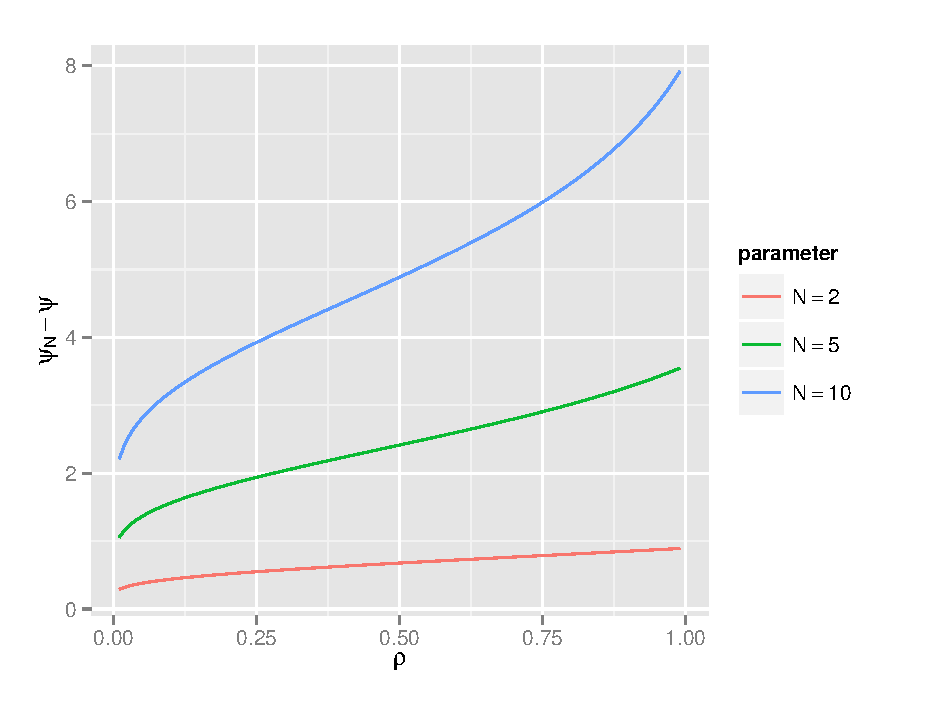
\includegraphics[width=14cm]{backorder_diff.eps}
\caption{改进前后极限成本率之差随$\rho$的变化}
\label{fig:改进前后极限成本率之差}
\end{figure}

图\ref{fig:改进前后极限成本率之差}显示,$\rho$越接近1,改进前后的库存之差越大。我们求出$\rho$接近1时,$\Delta\psi$的极限,可以作为改进效果的上限。设所有需求的到达速率相同,即$p_i=\frac{1}{N}$。
\begin{equation}
\lim_{\rho\to 1}\Delta\psi = h\ln\gamma\lim_{\rho\to 1}\sum_{i=1}^N\left[\frac{1}{\ln\frac{p_i\rho}{1-\rho+p_i\rho}}-\frac{p_i}{\ln\rho}\right]
\label{eq:极限成本率差}
\end{equation}
对公式\ref{eq:极限成本率差}使用洛必达法则,可以得到
\begin{equation}
\lim_{\rho\to 1}\Delta\psi = \frac{1}{2}h(N-1)\ln\frac{h+b}{h}
\label{eq:极限成本率差结果}
\end{equation}
公式\ref{eq:极限成本率差结果}可以作为估算改进效果上限的一种手段。







\section{服务水平约束的影响}

见文献《On the benefits of ...》







%%本章讨论提前期对改进效果的影响

\chapter{提前期对改进效果的影响}

\section{需求正态分布的情况}

仍然以汽车保险杠生产为例。假设生产一个注塑件耗时$\tau_1$,喷涂一个注塑件耗时$\tau_2$。客户允许的备货时间是$\tau$。

$\tau_1$、$\tau_2$、$\tau$三者的大小关系发生变化的时候,方案的改进效果也会发生变化。

(此处需要分类讨论很多条)



\section{需求泊松到达的情况}

设需求到达的速率为$\lambda_1$、$\lambda_2$,注塑速率$\mu_1$,喷涂速率$\mu_2$。建模成马尔科夫(生灭问题),可以求稳态概率,State 0 的概率即为缺货概率。

需要证明两个独立的泊松流合并后仍然是泊松流,且到达速率为$\lambda_1+\lambda_2$。

还需证明两个输入输出均为泊松过程的服务台,可以合并视为一个泊松过程的服务台(参考Jackson网络相关章节)。





\section{(s,S)库存策略下的情况}

由于换模等因素的影响,企业的实际生产中不可能随时对某种产品补货。往往采用的是(s,S)策略,即库存降到s后开始生产该产品,一直补货到库存为S为止。这种策略下也能建模成马尔科夫模型。




\chapter{总结与展望}





\section{总结}

本文主要从四个不同的方面探究了“合并同型号成品库存到在制品库存”这一改进方案可能产生的效果。本文在探究过程中采用的主要方式是数学建模,这使得本文的结论具有一定的局限性——基于很多理想化的假设条件;但同时也赋予了这些结论更强的普适性——没有局限于某个具体的企业生产线,而是给出普遍意义的结论。

在研究改进方案是否能够起到改进效果时,本文从数学性质良好的正态分布入手,证明了改进方案的优化潜力。还通过数值实验,研究了系统中一些参数对改进效果的影响。结果表明,需求波动越大、对服务水平要求越高的企业,在改进中获得的收益越大。

在研究改进失效现象时,本文既分析了数学性质良好的对称稳定分布,又分析了实际经常使用的右偏斜分布。同时也关注了服务水平的影响,探讨了两种不同的服务水平定义带来的不同结果。最后通过数值实验,找出参数影响改进失效现象的规律,提出了避免改进失效的方法,并且验证了之前证明的一些结论。

在研究需求相关性对改进效果的影响时,本文关注了很多文献都不曾注意的细节,把证明的基础建立在严密的构造上。讨论了极端状态下的改进效果,找到了需求相关性对改进效果的影响规律。得到结论后,又通过一些实际的数据为例,展示了企业应该如何利用这些结论来做决定。

研究延迟订单对改进效果的影响时,本文采用了运筹学的一些方法和结论,得到了定性和定量的结果。同时,还给出了估算改进效果上限的方法,为企业的决策提供一个参考。







\section{展望}

本文对需求分布、服务水平、生产时间等参数都有一定的研究,但尚未进展到对提前期变化的研究。企业将成品的库存合并前移到在制品,那么从在制品到成品所需的生产时间势必对改进效果产生相当重要的影响。再加上提前期的波动,整个系统在时间方面可能受到很大的影响。这一部分的研究也是比较有难度的。对时间问题的讨论可能需要继续使用马尔科夫过程,必要的时候还可能需要用到杰克逊网络。

除此之外,本文也没有涉及库存策略的影响。实际生产中对库存的控制往往是通过各种既定的策略来完成的,比如(s,S)策略,推动式生产或拉动式生产等等。当库存遵循这些策略的时候,改进方案还能起到效果吗?为了适应改进方案,库存策略中的一些参数应该取何值?

以上这些问题都是具有较强实际意义的,同时,它们也具有比较高的难度。若时间和精力允许,我将在未来的研究中尝试解决它们。

































%%% 其它部分
\backmatter

% 本科生要这几个索引,研究生不要。选择性留下。
\makeatletter
\ifthu@bachelor
  % 插图索引
  \listoffigures
  % 表格索引
  \listoftables
  % 公式索引
  \listofequations
\fi
\makeatother


% 参考文献
\bibliographystyle{thubib}
\bibliography{ref/refs}


% 致谢

%%% Local Variables:
%%% mode: latex
%%% TeX-master: "../main"
%%% End:

\begin{ack}

衷心感谢导师吴甦老师对我的帮助和指导。吴老师在选题和整体研究思路方面给了我很大的启发,为我的研究搭起了基本的框架。在完成这篇论文的过程中,吴老师始终尊重和鼓励我,为我答疑解惑而又不干涉我的想法。

感谢开题和中期答辩的评委皋琴老师、朱万山老师、曹晖老师,你们提出了很多宝贵的意见和建议,不仅修正了论文中可能出现的一些错误,也启发了很多新的思路和方法。

感谢吴振卿学长和陈昌国学长,你们在论文写作过程中给予了我很多实质性的帮助和建议。

感谢这篇论文所涉及到的各位学者,你们的研究使我受益良多,既是坚固的基石,又是灵感的源泉。

感谢父母、朋友和同学对我的关心,你们使我的生活更加精彩,使我能够以更饱满的热情投入到论文的写作中。

感谢\LaTeX 模板 \thuthesis,为我省去了调整论文格式的繁琐过程,使我能够专注于论文内容的写作。

\end{ack}


% 附录
\begin{appendix}
%%% Local Variables: 
%%% mode: latex
%%% TeX-master: "../main"
%%% End: 

\chapter{外文资料原文}
\label{cha:engorg}
As one of the most widely used techniques in operations research, {\em
  mathematical programming} is defined as a means of maximizing a quantity known
as {\em objective function}, subject to a set of constraints represented by
equations and inequalities. Some known subtopics of mathematical programming are
linear programming, nonlinear programming, multiobjective programming, goal
programming, dynamic programming, and multilevel programming$^{[1]}$.

It is impossible to cover in a single chapter every concept of mathematical
programming. This chapter introduces only the basic concepts and techniques of
mathematical programming such that readers gain an understanding of them
throughout the book$^{[2,3]}$.


\section{Single-Objective Programming}
The general form of single-objective programming (SOP) is written
as follows,
\begin{equation}\tag*{(123)} % 如果附录中的公式不想让它出现在公式索引中,那就请
                             % 用 \tag*{xxxx}
\left\{\begin{array}{l}
\max \,\,f(x)\\[0.1 cm]
\mbox{subject to:} \\ [0.1 cm]
\qquad g_j(x)\le 0,\quad j=1,2,\cdots,p
\end{array}\right.
\end{equation}
which maximizes a real-valued function $f$ of
$x=(x_1,x_2,\cdots,x_n)$ subject to a set of constraints.

\newtheorem{mpdef}{Definition}[chapter]
\begin{mpdef}
In SOP, we call $x$ a decision vector, and
$x_1,x_2,\cdots,x_n$ decision variables. The function
$f$ is called the objective function. The set
\begin{equation}\tag*{(456)} % 这里同理,其它不再一一指定。
S=\left\{x\in\Re^n\bigm|g_j(x)\le 0,\,j=1,2,\cdots,p\right\}
\end{equation}
is called the feasible set. An element $x$ in $S$ is called a
feasible solution.
\end{mpdef}

\newtheorem{mpdefop}[mpdef]{Definition}
\begin{mpdefop}
A feasible solution $x^*$ is called the optimal
solution of SOP if and only if
\begin{equation}
f(x^*)\ge f(x)
\end{equation}
for any feasible solution $x$.
\end{mpdefop}

One of the outstanding contributions to mathematical programming was known as
the Kuhn-Tucker conditions\ref{eq:ktc}. In order to introduce them, let us give
some definitions. An inequality constraint $g_j(x)\le 0$ is said to be active at
a point $x^*$ if $g_j(x^*)=0$. A point $x^*$ satisfying $g_j(x^*)\le 0$ is said
to be regular if the gradient vectors $\nabla g_j(x)$ of all active constraints
are linearly independent.

Let $x^*$ be a regular point of the constraints of SOP and assume that all the
functions $f(x)$ and $g_j(x),j=1,2,\cdots,p$ are differentiable. If $x^*$ is a
local optimal solution, then there exist Lagrange multipliers
$\lambda_j,j=1,2,\cdots,p$ such that the following Kuhn-Tucker conditions hold,
\begin{equation}
\label{eq:ktc}
\left\{\begin{array}{l}
    \nabla f(x^*)-\sum\limits_{j=1}^p\lambda_j\nabla g_j(x^*)=0\\[0.3cm]
    \lambda_jg_j(x^*)=0,\quad j=1,2,\cdots,p\\[0.2cm]
    \lambda_j\ge 0,\quad j=1,2,\cdots,p.
\end{array}\right.
\end{equation}
If all the functions $f(x)$ and $g_j(x),j=1,2,\cdots,p$ are convex and
differentiable, and the point $x^*$ satisfies the Kuhn-Tucker conditions
(\ref{eq:ktc}), then it has been proved that the point $x^*$ is a global optimal
solution of SOP.

\subsection{Linear Programming} 
\label{sec:lp}

If the functions $f(x),g_j(x),j=1,2,\cdots,p$ are all linear, then SOP is called
a {\em linear programming}.

The feasible set of linear is always convex. A point $x$ is called an extreme
point of convex set $S$ if $x\in S$ and $x$ cannot be expressed as a convex
combination of two points in $S$. It has been shown that the optimal solution to
linear programming corresponds to an extreme point of its feasible set provided
that the feasible set $S$ is bounded. This fact is the basis of the {\em simplex
  algorithm} which was developed by Dantzig as a very efficient method for
solving linear programming.
\begin{table}[ht]
\centering
  \centering
  \caption*{Table~1\hskip1em This is an example for manually numbered table, which
    would not appear in the list of tables}
  \label{tab:badtabular2}
  \begin{tabular}[c]{|c|m{0.8in}|c|c|c|c|c|}\hline
    \multicolumn{2}{|c|}{Network Topology} & \# of nodes & 
    \multicolumn{3}{c|}{\# of clients} & Server \\\hline
    GT-ITM & Waxman Transit-Stub & 600 &
    \multirow{2}{2em}{2\%}& 
    \multirow{2}{2em}{10\%}& 
    \multirow{2}{2em}{50\%}& 
    \multirow{2}{1.2in}{Max. Connectivity}\\\cline{1-3}
    \multicolumn{2}{|c|}{Inet-2.1} & 6000 & & & &\\\hline
    \multirow{2}{1in}{Xue} & Rui  & Ni &\multicolumn{4}{c|}{\multirow{2}*{\thuthesis}}\\\cline{2-3}
    & \multicolumn{2}{c|}{ABCDEF} &\multicolumn{4}{c|}{} \\\hline
\end{tabular}  
\end{table}

Roughly speaking, the simplex algorithm examines only the extreme points of the
feasible set, rather than all feasible points. At first, the simplex algorithm
selects an extreme point as the initial point. The successive extreme point is
selected so as to improve the objective function value. The procedure is
repeated until no improvement in objective function value can be made. The last
extreme point is the optimal solution.

\subsection{Nonlinear Programming}

If at least one of the functions $f(x),g_j(x),j=1,2,\cdots,p$ is nonlinear, then
SOP is called a {\em nonlinear programming}.

A large number of classical optimization methods have been developed to treat
special-structural nonlinear programming based on the mathematical theory
concerned with analyzing the structure of problems.
\begin{figure}[h]
  \centering
  \includegraphics[clip]{thu-lib-logo}
  \caption*{Figure~1\hskip1em This is an example for manually numbered figure,
    which would not appear in the list of figures}
  \label{tab:badfigure2}    
\end{figure}

Now we consider a nonlinear programming which is confronted solely with
maximizing a real-valued function with domain $\Re^n$.  Whether derivatives are
available or not, the usual strategy is first to select a point in $\Re^n$ which
is thought to be the most likely place where the maximum exists. If there is no
information available on which to base such a selection, a point is chosen at
random. From this first point an attempt is made to construct a sequence of
points, each of which yields an improved objective function value over its
predecessor. The next point to be added to the sequence is chosen by analyzing
the behavior of the function at the previous points. This construction continues
until some termination criterion is met. Methods based upon this strategy are
called {\em ascent methods}, which can be classified as {\em direct methods},
{\em gradient methods}, and {\em Hessian methods} according to the information
about the behavior of objective function $f$. Direct methods require only that
the function can be evaluated at each point. Gradient methods require the
evaluation of first derivatives of $f$. Hessian methods require the evaluation
of second derivatives. In fact, there is no superior method for all
problems. The efficiency of a method is very much dependent upon the objective
function.

\subsection{Integer Programming}

{\em Integer programming} is a special mathematical programming in which all of
the variables are assumed to be only integer values. When there are not only
integer variables but also conventional continuous variables, we call it {\em
  mixed integer programming}. If all the variables are assumed either 0 or 1,
then the problem is termed a {\em zero-one programming}. Although integer
programming can be solved by an {\em exhaustive enumeration} theoretically, it
is impractical to solve realistically sized integer programming problems. The
most successful algorithm so far found to solve integer programming is called
the {\em branch-and-bound enumeration} developed by Balas (1965) and Dakin
(1965). The other technique to integer programming is the {\em cutting plane
  method} developed by Gomory (1959).

\hfill\textit{Uncertain Programming\/}\quad(\textsl{BaoDing Liu, 2006.2})

\section*{References}
\noindent{\itshape NOTE: these references are only for demonstration, they are
  not real citations in the original text.}

\begin{enumerate}[{$[$}1{$]$}]
\item Donald E. Knuth. The \TeX book. Addison-Wesley, 1984. ISBN: 0-201-13448-9
\item Paul W. Abrahams, Karl Berry and Kathryn A. Hargreaves. \TeX\ for the
  Impatient. Addison-Wesley, 1990. ISBN: 0-201-51375-7
\item David Salomon. The advanced \TeX book.  New York : Springer, 1995. ISBN:0-387-94556-3
\end{enumerate}

\chapter{外文资料的调研阅读报告或书面翻译}
\section{单目标规划}
北冥有鱼,其名为鲲。鲲之大,不知其几千里也。化而为鸟,其名为鹏。鹏之背,不知其几
千里也。怒而飞,其翼若垂天之云。是鸟也,海运则将徙于南冥。南冥者,天池也。 
\begin{equation}\tag*{(123)}
 p(y|\mathbf{x}) = \frac{p(\mathbf{x},y)}{p(\mathbf{x})}=
\frac{p(\mathbf{x}|y)p(y)}{p(\mathbf{x})}
\end{equation}

吾生也有涯,而知也无涯。以有涯随无涯,殆已!已而为知者,殆而已矣!为善无近名,为
恶无近刑,缘督以为经,可以保身,可以全生,可以养亲,可以尽年。

\subsection{线性规划}
庖丁为文惠君解牛,手之所触,肩之所倚,足之所履,膝之所倚,砉然响然,奏刀騞然,莫
不中音,合于桑林之舞,乃中经首之会。
\begin{table}[ht]
\centering
  \centering
  \caption*{表~1\hskip1em 这是手动编号但不出现在索引中的一个表格例子}
  \label{tab:badtabular3}
  \begin{tabular}[c]{|c|m{0.8in}|c|c|c|c|c|}\hline
    \multicolumn{2}{|c|}{Network Topology} & \# of nodes & 
    \multicolumn{3}{c|}{\# of clients} & Server \\\hline
    GT-ITM & Waxman Transit-Stub & 600 &
    \multirow{2}{2em}{2\%}& 
    \multirow{2}{2em}{10\%}& 
    \multirow{2}{2em}{50\%}& 
    \multirow{2}{1.2in}{Max. Connectivity}\\\cline{1-3}
    \multicolumn{2}{|c|}{Inet-2.1} & 6000 & & & &\\\hline
    \multirow{2}{1in}{Xue} & Rui  & Ni &\multicolumn{4}{c|}{\multirow{2}*{\thuthesis}}\\\cline{2-3}
    & \multicolumn{2}{c|}{ABCDEF} &\multicolumn{4}{c|}{} \\\hline
\end{tabular}  
\end{table}

文惠君曰:“嘻,善哉!技盖至此乎?”庖丁释刀对曰:“臣之所好者道也,进乎技矣。始臣之
解牛之时,所见无非全牛者;三年之后,未尝见全牛也;方今之时,臣以神遇而不以目视,
官知止而神欲行。依乎天理,批大郤,导大窾,因其固然。技经肯綮之未尝,而况大坬乎!
良庖岁更刀,割也;族庖月更刀,折也;今臣之刀十九年矣,所解数千牛矣,而刀刃若新发
于硎。彼节者有间而刀刃者无厚,以无厚入有间,恢恢乎其于游刃必有余地矣。是以十九年
而刀刃若新发于硎。虽然,每至于族,吾见其难为,怵然为戒,视为止,行为迟,动刀甚微,
謋然已解,如土委地。提刀而立,为之而四顾,为之踌躇满志,善刀而藏之。”

文惠君曰:“善哉!吾闻庖丁之言,得养生焉。”


\subsection{非线性规划}
孔子与柳下季为友,柳下季之弟名曰盗跖。盗跖从卒九千人,横行天下,侵暴诸侯。穴室枢
户,驱人牛马,取人妇女。贪得忘亲,不顾父母兄弟,不祭先祖。所过之邑,大国守城,小
国入保,万民苦之。孔子谓柳下季曰:“夫为人父者,必能诏其子;为人兄者,必能教其弟。
若父不能诏其子,兄不能教其弟,则无贵父子兄弟之亲矣。今先生,世之才士也,弟为盗
跖,为天下害,而弗能教也,丘窃为先生羞之。丘请为先生往说之。”
\begin{figure}[h]
  \centering
  \includegraphics{hello}
  \caption*{图~1\hskip1em 这是手动编号但不出现索引中的图片的例子}
  \label{tab:badfigure3}    
\end{figure}

柳下季曰:“先生言为人父者必能诏其子,为人兄者必能教其弟,若子不听父之诏,弟不受
兄之教,虽今先生之辩,将奈之何哉?且跖之为人也,心如涌泉,意如飘风,强足以距敌,
辩足以饰非。顺其心则喜,逆其心则怒,易辱人以言。先生必无往。”

孔子不听,颜回为驭,子贡为右,往见盗跖。

\subsection{整数规划}
盗跖乃方休卒徒大山之阳,脍人肝而餔之。孔子下车而前,见谒者曰:“鲁人孔丘,闻将军
高义,敬再拜谒者。”谒者入通。盗跖闻之大怒,目如明星,发上指冠,曰:“此夫鲁国之
巧伪人孔丘非邪?为我告之:尔作言造语,妄称文、武,冠枝木之冠,带死牛之胁,多辞缪
说,不耕而食,不织而衣,摇唇鼓舌,擅生是非,以迷天下之主,使天下学士不反其本,妄
作孝弟,而侥幸于封侯富贵者也。子之罪大极重,疾走归!不然,我将以子肝益昼餔之膳。”


\chapter{其它附录}
前面两个附录主要是给本科生做例子。其它附录的内容可以放到这里,当然如果你愿意,可
以把这部分也放到独立的文件中,然后将其 \verb|\input| 到主文件中。
\end{appendix}

% 个人简历
%\begin{resume}

  \resumeitem{个人简历}

  xxxx 年 xx 月 xx 日出生于 xx 省 xx 县。
  
  xxxx 年 9 月考入 xx 大学 xx 系 xx 专业,xxxx 年 7 月本科毕业并获得 xx 学士学位。
  
  xxxx 年 9 月免试进入 xx 大学 xx 系攻读 xx 学位至今。

  \resumeitem{发表的学术论文} % 发表的和录用的合在一起

  \begin{enumerate}[{[}1{]}]
  \item Yang Y, Ren T L, Zhang L T, et al. Miniature microphone with silicon-
    based ferroelectric thin films. Integrated Ferroelectrics, 2003,
    52:229-235. (SCI 收录, 检索号:758FZ.)
  \item 杨轶, 张宁欣, 任天令, 等. 硅基铁电微声学器件中薄膜残余应力的研究. 中国机
    械工程, 2005, 16(14):1289-1291. (EI 收录, 检索号:0534931 2907.)
  \item 杨轶, 张宁欣, 任天令, 等. 集成铁电器件中的关键工艺研究. 仪器仪表学报,
    2003, 24(S4):192-193. (EI 源刊.)
  \item Yang Y, Ren T L, Zhu Y P, et al. PMUTs for handwriting recognition. In
    press. (已被 Integrated Ferroelectrics 录用. SCI 源刊.)
  \item Wu X M, Yang Y, Cai J, et al. Measurements of ferroelectric MEMS
    microphones. Integrated Ferroelectrics, 2005, 69:417-429. (SCI 收录, 检索号
    :896KM.)
  \item 贾泽, 杨轶, 陈兢, 等. 用于压电和电容微麦克风的体硅腐蚀相关研究. 压电与声
    光, 2006, 28(1):117-119. (EI 收录, 检索号:06129773469.)
  \item 伍晓明, 杨轶, 张宁欣, 等. 基于MEMS技术的集成铁电硅微麦克风. 中国集成电路, 
    2003, 53:59-61.
  \end{enumerate}

  \resumeitem{研究成果} % 有就写,没有就删除
  \begin{enumerate}[{[}1{]}]
  \item 任天令, 杨轶, 朱一平, 等. 硅基铁电微声学传感器畴极化区域控制和电极连接的
    方法: 中国, CN1602118A. (中国专利公开号.)
  \item Ren T L, Yang Y, Zhu Y P, et al. Piezoelectric micro acoustic sensor
    based on ferroelectric materials: USA, No.11/215, 102. (美国发明专利申请号.)
  \end{enumerate}
\end{resume}


%书脊
\shuji


\end{document}
